% ============================================================
%  MEMORIA PRINCIPAL - DocumentChain
%  Sistema de Gestion Documental mediante Blockchain
%  Universidad de Salamanca - Grado en Ingenieria Informatica
% ============================================================
\documentclass[11pt, a4paper]{article}

\usepackage{fontspec}
\usepackage[spanish]{babel}
\usepackage{graphicx}
\graphicspath{{diagramas/}{capturas-ui/}}
\usepackage{float}
\usepackage{amsmath}
\usepackage{xcolor}
\usepackage[protrusion=true,expansion=false]{microtype}
\usepackage{longtable}
\usepackage{array}
\usepackage{booktabs}
\usepackage{multirow}
\usepackage{enumitem}
\usepackage{listings}
\usepackage{pdflscape}
\usepackage[
    colorlinks = true,
    linkcolor  = black,
    urlcolor   = black,
    citecolor  = black
]{hyperref}
\usepackage{geometry}
\geometry{left=2.5cm, right=2.5cm, top=3cm, bottom=2.5cm, headheight=55pt, headsep=0.8cm}
\usepackage{fancyhdr}
\pagestyle{fancy}
\fancyhf{}
\lhead{
\includegraphics[height=1.25cm]{USAL-Logo-3820702873.png}}
\rhead{\shortstack[r]{\fontsize{10}{12}\selectfont\textbf{Memoria}\\[-1pt]\fontsize{10}{12}\selectfont DocumentChain}}
\renewcommand{\headrulewidth}{0pt}
\renewcommand{\footrulewidth}{0pt}
\cfoot{%
    \color{gray}\rule[0.5ex]{0.4\textwidth}{0.8pt}%
    \hspace{0.5cm}%
    \textcolor{black}{\textbf{\thepage}}%
    \hspace{0.5cm}%
    \color{gray}\rule[0.5ex]{0.4\textwidth}{0.8pt}%
}

\definecolor{lightgray}{rgb}{0.96, 0.96, 0.96}
\definecolor{darkblue}{rgb}{0.0, 0.0, 0.6}
\definecolor{darkorange}{rgb}{0.8, 0.4, 0.0}
\lstset{
    basicstyle=\ttfamily\scriptsize,
    breaklines=true, frame=single,
    backgroundcolor=\color{lightgray},
    keywordstyle=\color{darkblue}\bfseries,
    stringstyle=\color{darkorange},
    showstringspaces=false,
}
\lstdefinelanguage{JavaScript}{
    keywords={break,case,catch,class,const,continue,debugger,default,delete,do,
              else,export,extends,false,finally,for,function,if,import,in,
              instanceof,let,new,null,return,super,switch,this,throw,true,try,
              typeof,var,void,while,with,yield,async,await,from,of},
    sensitive=true,
    comment=[l]{//},
    morecomment=[s]{/*}{*/},
    morestring=[b]',
    morestring=[b]",
    morestring=[b]`,
}

\newcommand{\tituloInforme}{DocumentChain}
\newcommand{\subtituloInforme}{Sistema de Gestion Documental mediante Blockchain}
\newcommand{\asignatura}{Trabajo de Fin de Grado}
\newcommand{\autorUno}{David Pérez Velasco}
\newcommand{\tutorUno}{Gabriel Villarrubia González}
\newcommand{\tutorDos}{Sergio García González}

\begin{document}

% ============================================================
% PORTADA
% ============================================================
\begin{titlepage}
    \centering
    \vspace*{1.5cm}
    {\scshape\LARGE Universidad de Salamanca \par}
    \vspace{1cm}
    {\scshape\Large Grado en Ingenieria Informatica \par}
    \vspace{1.5cm}
    {\huge\bfseries \tituloInforme \par}
    \vspace{0.5cm}
    {\Large\bfseries \subtituloInforme \par}
    \vspace{1.8cm}
    
\includegraphics[width=0.28\textwidth]{USAL-Logo-3820702873.png}

    \vspace{2.2cm}

    {\Large\itshape \autorUno \par}
    \vspace{1.5cm}
    {\large Tutores: \par}
    \vspace{0.3cm}
    {\large \tutorUno \par}
    \vspace{0.2cm}
    {\large \tutorDos \par}

    \vspace{2cm}
    {\large Julio 2026}
    \vspace{0.5cm}

    {Trabajo de Fin de Grado \par}
    \vspace{1cm}
\end{titlepage}

% ============================================================
% CONSENTIMIENTO INFORMADO
% ============================================================
\newpage
\thispagestyle{empty}
\vspace*{3cm}
\begin{center}
    {\Large\bfseries Consentimiento informado del tutor \par}
\end{center}
\vspace{2cm}

El Dr. \tutorUno, profesor del Departamento de Informatica y Automatica de la Universidad de Salamanca, y el Dr. \tutorDos, certifican que el trabajo titulado ``\tituloInforme: \subtituloInforme'' ha sido realizado por D. \autorUno, y constituye el trabajo realizado de cara a la superacion de la asignatura Trabajo de Fin de Grado de la titulacion Grado Universitario en Ingenieria Informatica de la Universidad de Salamanca.

\vspace{3cm}
\begin{flushright}
    En Salamanca, a \rule{4cm}{0.4pt}
    \vspace{1cm}

    Fdo.: \tutorUno
    \vspace{0.5cm}

    Fdo.: \tutorDos
\end{flushright}

% ============================================================
% RESUMEN
% ============================================================
\newpage
\section*{Resumen}
\addcontentsline{toc}{section}{Resumen}

Los sistemas de gestion documental convencionales ofrecen control de versiones y comparticion, pero carecen de mecanismos descentralizados que garanticen la inmutabilidad del contenido y la verificacion criptografica de las operaciones, por lo que la autenticidad y la trazabilidad siguen siendo problemas sin resolver.

Ante esta problematica surge \textbf{DocumentChain}, un sistema de gestion documental que integra tecnologia blockchain para garantizar la autenticidad, trazabilidad e inmutabilidad de los documentos gestionados. El proyecto combina una aplicacion web desarrollada con React y TypeScript, una API REST con Node.js y Express, y una capa de almacenamiento distribuido mediante IPFS. La blockchain local (Hardhat) registra los hashes de contenido y las firmas digitales, proporcionando un historial inmutable de operaciones.

El sistema implementa un esquema de seguridad por capas (autenticacion JWT con verificacion de email, cifrado AES-256-GCM con intercambio ECDH y registro blockchain verificable), soporta la firma digital mediante wallets compatibles con EIP-6963 y ofrece un mecanismo de verificacion publica accesible sin autenticacion. El resultado es una plataforma funcional que demuestra la viabilidad tecnica de combinar gestion documental con trazabilidad descentralizada, sentando las bases para futuras mejoras y ampliaciones.

\textbf{Palabras clave}: gestion documental, blockchain, autenticidad, firma digital, IPFS, cifrado, trazabilidad, descentralizacion.

\vspace{1cm}

% ============================================================
% ABSTRACT
% ============================================================
\section*{Abstract}
\addcontentsline{toc}{section}{Abstract}

In the field of digital document management, authenticity and traceability represent critical challenges that traditional solutions fail to address satisfactorily. Conventional cloud storage systems offer versioning and sharing capabilities, but lack decentralized mechanisms that guarantee content immutability and cryptographic verification of performed operations.

In response to this problem, \textbf{DocumentChain} emerges as a document management system that integrates blockchain technology to ensure the authenticity, traceability and immutability of managed documents. The project combines a web application developed with React and TypeScript, a REST API with Node.js and Express, and a distributed storage layer through IPFS. The local blockchain (Hardhat) registers content hashes and digital signatures, providing an immutable history of operations.

The system implements a layered security scheme (JWT-based authentication with email verification, AES-256-GCM encryption with ECDH key exchange, and verifiable blockchain registry), supports digital signing through EIP-6963 compatible wallets, and offers a public verification mechanism accessible without authentication. The result is a functional platform that demonstrates the technical feasibility of combining document management with decentralized traceability, laying the groundwork for future improvements and extensions.

\textbf{Keywords}: document management, blockchain, authenticity, digital signature, IPFS, encryption, traceability, decentralization.

% ============================================================
% INDICES
% ============================================================
\newpage
\tableofcontents
\newpage
\listoffigures
\newpage
\listoftables
\newpage

% ============================================================
% GLOSARIO
% ============================================================
\section*{Glosario}
\addcontentsline{toc}{section}{Glosario}

\begin{description}[style=nextline]
    \item[API (Application Programming Interface)] Conjunto de definiciones y protocolos que permiten la comunicacion entre diferentes componentes software.
    \item[Blockchain] Estructura de datos distribuida e inmutable compuesta por bloques enlazados mediante funciones hash.
    \item[CID (Content Identifier)] Identificador unico de contenido en IPFS basado en hashing criptografico.
    \item[ECDH (Elliptic Curve Diffie-Hellman)] Protocolo de intercambio de claves basado en curvas elipticas.
    \item[EIP-6963] Propuesta de mejora de Ethereum para la deteccion de wallets mediante eventos de ventana.
    \item[personal\_sign] Metodo de firma de mensajes arbitrarios mediante una wallet Ethereum, empleado para acreditar la posesion de la direccion que firma una operacion.
    \item[IPFS (InterPlanetary File System)] Protocolo descentralizado de almacenamiento y distribucion de archivos.
    \item[JWT (JSON Web Token)] Token firmado digitalmente utilizado para la autenticacion entre partes.
    \item[SPA (Single Page Application)] Aplicacion web que carga una unica pagina HTML y actualiza el contenido dinamicamente.
    \item[TOTP (Time-based One-Time Password)] Contrasena de un solo uso basada en tiempo para autenticacion multifactor (no implementada en la version actual del sistema).
    \item[UCP (Use Case Points)] Tecnica de estimacion del tamano y esfuerzo de proyectos software basada en casos de uso.
    \item[EVM (Ethereum Virtual Machine)] Maquina virtual que ejecuta smart contracts en la red Ethereum.
\end{description}

\newpage

% ============================================================
% CAPITULO 1: INTRODUCCION
% ============================================================

% ============================================================
% CAPITULO 1: INTRODUCCION
% ============================================================
\section{Introduccion}

\subsection{Contexto y motivacion}

La digitalizacion ha cambiado por completo la forma en que gestionamos la informacion. Herramientas como Google Drive o Dropbox permiten compartir archivos y mantener un historial de versiones, pero tienen un problema de fondo: todo depende de un unico proveedor. Si ese proveedor modifica un archivo, lo censura o simplemente cierra el servicio, el usuario se queda sin garantias.

La tecnologia blockchain ofrece una alternativa interesante a este modelo. Al mantener un registro descentralizado que nadie puede modificar unilateralmente, permite guardar huellas digitales de los documentos de forma que cualquiera pueda verificar su autenticidad sin necesidad de confiar en un tercero. Esto fue lo que motivo este trabajo: comprobar si era viable construir una plataforma de gestion documental donde la prueba de autenticidad no dependa de la palabra de una empresa, sino de las matematicas.

\subsection{Problematica actual}

El problema de la autenticidad documental va mas alla de lo tecnologico. Hoy en dia modificar un PDF o un titulo academico es sorprendentemente facil, y las victimas de estas falsificaciones a menudo no tienen forma de demostrarlo. Los sistemas de firma digital tradicionales existen, pero su adopcion es baja porque requieren certificados que son complicados de gestionar para el usuario medio.

A esto se le suma que los sistemas de almacenamiento actuales son cajas negras: el proveedor controla los registros de auditoria y el usuario no puede comprobar por si mismo si un documento ha sido alterado. Las filtraciones masivas de datos de los ultimos anos demuestran que confiar toda la informacion a un unico servidor no es la mejor estrategia.

\subsection{Solucion propuesta}

DocumentChain es una plataforma web que combina tres tecnologias para resolver estos problemas. Por un lado, usa blockchain para registrar huellas inmutables de cada documento. Por otro, emplea IPFS como almacenamiento descentralizado, donde los archivos se identifican por su contenido y no por el servidor que los aloja. Y por ultimo, cifra los documentos privados de extremo a extremo para que ni siquiera el servidor pueda leer su contenido.

La aplicacion se ha construido con React y TypeScript en el frontend, Node.js y Express en el backend, PostgreSQL para los datos operativos y contratos inteligentes en Solidity para el registro en blockchain. El usuario firma las operaciones con su wallet (compatible con EIP-6963) y el sistema permite que cualquier persona, sin necesidad de crear una cuenta, verifique si un documento es autentico consultando directamente la blockchain.

\subsection{Estructura del documento}

El presente documento se organiza en diez capitulos. El Capitulo 1 introduce el contexto, la problematica, la solucion propuesta y la estructura del documento. El Capitulo 2 recoge un estudio de mercado con el analisis de soluciones comerciales, sus deficiencias, la propuesta diferenciadora de DocumentChain y la investigacion academica de referencia. Los objetivos funcionales y personales del proyecto se detallan en el Capitulo 3. El Capitulo 4 expone los conceptos teoricos: autenticidad documental, marco legal, impacto economico, necesidad de descentralizacion y tecnologias habilitadoras. A continuacion, el Capitulo 5 describe las herramientas de desarrollo, los estandares empleados y el uso de inteligencia artificial. El Capitulo 6 aborda los aspectos mas relevantes del desarrollo, desde el marco de trabajo y la estimacion hasta la planificacion, los requisitos, el analisis, el diseno, la implementacion y la funcionalidad resultante. Las limitaciones de tiempo, tecnologicas, de seguridad y de acceso a usuarios se tratan en el Capitulo 7. El Capitulo 8 presenta las conclusiones del proyecto, con la validacion de los objetivos alcanzados y una reflexion sobre el trabajo realizado. Las lineas de trabajo futuras y las mejoras propuestas para la evolucion del sistema figuran en el Capitulo 9. Por ultimo, el Capitulo 10 recopila las fuentes consultadas en formato estandarizado.

\noindent Para completar la explicacion de esta memoria, se acompana de nueve anexos donde se recoge la documentacion tecnica exhaustiva. El Anexo I contiene el catalogo completo de requisitos funcionales, no funcionales y de informacion, junto con los actores, los diagramas de casos de uso y la matriz de rastreabilidad. El Anexo II detalla la metodologia de estimacion, el calculo de Use Case Points, la planificacion temporal y los diagramas de Gantt. El Anexo III documenta el analisis y diseno del sistema: modelo de dominio, diagramas BCE, arquitectura, clases de diseno, base de datos y modelo de despliegue. La documentacion tecnica del codigo, las tecnologias, los modulos, los smart contracts y la arquitectura de cifrado se recogen en el Anexo IV. El Anexo V presenta el plan de seguridad con los activos criticos, las amenazas, la matriz de riesgos y las medidas implementadas. El Anexo VI es el manual de usuario, con la guia de instalacion, configuracion y uso paso a paso de la aplicacion. El Anexo VII constituye el manual de montaje y despliegue, con los requisitos, la instalacion mediante Docker Compose y la verificacion del despliegue. La declaracion de las herramientas de inteligencia artificial empleadas y la transparencia en su uso se documentan en el Anexo VIII. Por ultimo, el Anexo IX expone la metodologia de Diseno Centrado en el Usuario aplicada para asegurar la usabilidad del sistema.

\subsection{Participantes del proyecto}

El presente Trabajo de Fin de Grado ha sido desarrollado en el marco de la asignatura Trabajo de Fin de Grado del Grado en Ingenieria Informatica de la Universidad de Salamanca durante el curso academico 2025-2026. Los participantes en el proyecto son:

\begin{itemize}
    \item \textbf{Autor}: D. David Perez Velasco, alumno del Grado en Ingenieria Informatica de la Universidad de Salamanca, responsable del analisis, diseno, implementacion, documentacion y despliegue del sistema DocumentChain.
    \item \textbf{Tutor academico}: Dr. D. Gabriel Villarrubia Gonzalez, profesor del Departamento de Informatica y Automatica de la Universidad de Salamanca, responsable de la supervision tecnica y metodologica del proyecto.
    \item \textbf{Cotutor}: Dr. D. Sergio Garcia Gonzalez, responsable de la supervision complementaria del desarrollo y la documentacion del sistema.
\end{itemize}

% ============================================================
% CAPITULO 2: ESTUDIO DE MERCADO
% ============================================================
\section{Estudio de mercado}

En este apartado se ha realizado un estudio de las soluciones comerciales existentes con el fin de identificar sus carencias y establecer una propuesta diferenciadora para DocumentChain.

\subsection{Aplicaciones comerciales existentes}

Antes de comenzar el desarrollo, se llevo a cabo un estudio del mercado disponible tratando de encontrar productos similares u orientados al mismo proposito. Se analizaron cuatro productos comerciales y una linea de investigacion academica.

\textbf{DocuSign} es el actor dominante en firma electronica, operando bajo un modelo SaaS centralizado. Ofrece flujos de trabajo configurables y cumplimiento con eIDAS, pero su funcion principal gira en torno a la firma, no al ciclo de vida documental completo. La arquitectura centralizada implica que DocuSign actua como unico guardian de la verdad, por lo que no permite la verificacion independiente por terceros.

\textbf{Adobe Sign} se integra con Adobe Document Cloud y soporta firmas cualificadas. Comparte las limitaciones de DocuSign: centralizacion, ausencia de blockchain y dependencia del proveedor, por lo que presenta los mismos problemas de confianza que el anterior.

\textbf{Google Drive y Dropbox} ofrecen almacenamiento, sincronizacion y control de versiones basico. Sin embargo, su proposito es la productividad, no la garantia de autenticidad, por lo que los registros pueden ser modificados por el administrador sin dejar rastro.

\textbf{OriginStamp} adopta un enfoque de \textit{proof of existence} registrando hashes en la blockchain de Bitcoin. No almacena documentos ni gestiona permisos, por lo que resulta insuficiente para una gestion documental completa.

\subsection{Deficiencias identificadas}

El analisis de las soluciones existentes revela deficiencias en cinco dimensiones: arquitectura de confianza centralizada con punto unico de fallo, ausencia de cifrado de extremo a extremo, registros de auditoria mutables, fragmentacion funcional que obliga a combinar multiples herramientas y modelos de precios que generan barreras para pequenas organizaciones. La Tabla \ref{tab:deficiencias} resume estas limitaciones.

\begin{table}[H]
\centering
\renewcommand{\arraystretch}{1.4}
\small
\begin{tabular}{|p{2.5cm}|p{3cm}|p{3cm}|p{3.5cm}|}
\hline
\textbf{Dimension} & \textbf{Deficiencia} & \textbf{Impacto} & \textbf{Soluciones afectadas} \\
\hline
Arquitectura de confianza & Dependencia de autoridad central unica & Riesgo de censura, suspension y punto unico de fallo & DocuSign, Adobe Sign, Drive, Dropbox \\
\hline
Seguridad del contenido & Ausencia de cifrado de extremo a extremo & El proveedor puede acceder al contenido & Todas las centralizadas \\
\hline
Trazabilidad historica & Registros de auditoria mutables & Imposibilidad de demostrar la secuencia real de operaciones & Todas excepto OriginStamp \\
\hline
Funcionalidad documental & Fragmentacion entre firma, almacenamiento y prueba & Necesidad de multiples herramientas & Todas \\
\hline
Coste y accesibilidad & Suscripcion por usuario o transaccion & Barrera para PYMEs y usuarios individuales & DocuSign, Adobe Sign \\
\hline
\end{tabular}
\caption{Deficiencias identificadas en las soluciones comerciales actuales}
\label{tab:deficiencias}
\end{table}

\subsection{Propuesta diferenciadora}

DocumentChain integra en una unica plataforma gestion documental, cifrado, almacenamiento distribuido y registro blockchain. A diferencia de las soluciones analizadas, no depende de un proveedor centralizado ni obliga a combinar varias herramientas, por lo que ofrece una experiencia mas unificada. La Tabla \ref{tab:ventajas} resume sus pilares diferenciadores.

\begin{table}[H]
\centering
\renewcommand{\arraystretch}{1.4}
\small
\begin{tabular}{|p{3.5cm}|p{4cm}|p{4.5cm}|}
\hline
\textbf{Pilar diferenciador} & \textbf{Descripcion tecnica} & \textbf{Ventaja competitiva} \\
\hline
Gestion documental completa & CRUD, carpetas, versiones, comparticion, transferencia & Ciclo de vida integral sin fragmentacion \\
\hline
Cifrado de extremo a extremo & AES-256-GCM con ECDH P-256 en el cliente & Confidencialidad incluso ante compromision del servidor \\
\hline
Almacenamiento distribuido & IPFS con CID & Resistencia a la censura y punto unico de fallo \\
\hline
Registro inmutable & Smart contracts con hashes SHA-256 y firmas mediante wallet & Trazabilidad verificable sin intermediarios \\
\hline
Verificacion publica & Endpoint abierto por hash o txHash & Transparencia universal sin registro previo \\
\hline
\end{tabular}
\caption{Pilares diferenciadores de DocumentChain}
\label{tab:ventajas}
\end{table}

\subsection{Investigacion academica relacionada}

La gestion documental descentralizada ha recibido creciente atencion academica. Zyskind, Nathan y Pentland (2015) proponen un sistema donde la blockchain actua como registro de control de acceso y los datos se almacenan off-chain, modelo adoptado por DocumentChain. Liang et al. (2017) presentan en ProvChain una arquitectura de trazabilidad de datos en la nube con registro blockchain de cada operacion. En cuanto al almacenamiento distribuido, Benet (2014) establece el protocolo IPFS que DocumentChain utiliza como capa de almacenamiento. La contribucion de este proyecto radica en integrar todas estas capacidades en un unico sistema documentado, funcional y reproducible.

% ============================================================
% CAPITULO 3: OBJETIVOS
% ============================================================
\section{Objetivos}

En este apartado se recogen los objetivos que el sistema debe cumplir para considerarse totalmente funcional, asi como los objetivos personales que se pretenden alcanzar con el desarrollo de este proyecto.

\subsection{Objetivos del sistema}

El objetivo principal del proyecto es disenar e implementar un sistema de gestion documental con trazabilidad blockchain que garantice la autenticidad, integridad y confidencialidad de los documentos mediante cifrado de extremo a extremo y registro inmutable. En particular, se definen los siguientes objetivos:

\begin{itemize}
    \item \textbf{Gestion documental completa}: permitir el ciclo de vida completo de los documentos digitales (crear, versionar, compartir, firmar, archivar y eliminar).
    \item \textbf{Registro inmutable en blockchain}: integrar una capa blockchain para el registro de hashes de documentos y firmas digitales, garantizando trazabilidad verificable.
    \item Que el sistema permita firmar documentos mediante wallets compatibles con EIP-6963, generando mensajes de firma mediante wallet y registrando la firma en blockchain.
    \item Se necesita un modulo de cifrado AES-256-GCM en el cliente, con intercambio de claves ECDH P-256, para que el contenido de los documentos privados resulte inaccesible incluso para el servidor.
    \item \textbf{Verificacion publica}: proporcionar un mecanismo de verificacion de autenticidad accesible sin necesidad de registro previo.
    \item \textbf{Panel de administracion}: disenar un panel para la gestion de usuarios, roles y supervision del sistema.
    \item \textbf{Documentacion exhaustiva}: documentar el sistema siguiendo la normativa CCII-N2016-02 de la Universidad de Salamanca.
\end{itemize}

\subsection{Objetivos personales}

\begin{itemize}
    \item \textbf{Profundizar en tecnologias blockchain}: adquirir competencia practica en el desarrollo de smart contracts y su integracion en aplicaciones web.
    \item \textbf{Desarrollo full-stack}: dominar un stack tecnologico moderno que abarca React, Node.js, Solidity, Docker e IPFS de forma coordinada.
    \item \textbf{Ingenieria del software}: aplicar metodologias de analisis, diseno y estimacion basadas en el Proceso Unificado y Use Case Points.
    \item \textbf{Gestion integral de proyectos}: demostrar la capacidad de conducir un proyecto complejo desde la concepcion hasta la documentacion final.
\end{itemize}

% ============================================================
% CAPITULO 4: CONCEPTOS TEORICOS
% ============================================================
\section{Conceptos teoricos}

En este apartado se abordan conceptos teoricos necesarios para el correcto entendimiento del proyecto, facilitando asi la lectura y comprension por parte del lector.

\subsection{Problemas de autenticidad documental}

La autenticidad de los documentos es un problema real y cotidiano. Modificar un PDF, un titulo universitario o un informe medico es sorprendentemente facil con las herramientas actuales, y las victimas rara vez pueden demostrarlo. Los sistemas de firma digital basados en PKI llevan anos intentando resolver esto, pero su complejidad (gestion de certificados, autoridades centralizadas) hace que pocas organizaciones pequenas los usen realmente.

\subsection{Marco legal europeo}

El sistema se ha disenado teniendo en cuenta dos normativas europeas. El reglamento eIDAS (UE 910/2014) establece tres niveles de firma electronica y da validez legal a las firmas digitales. El RGPD (UE 2016/679) obliga a proteger los datos personales. DocumentChain intenta cumplir ambos: los documentos privados viajan cifrados, en la blockchain solo se guardan hashes (no el contenido), y la recuperacion de archivos se hace por CID, sin depender de un proveedor concreto.

\subsection{Impacto economico y social de la falsificacion documental}

Las cifras son llamativas. Segun la Association of Certified Fraud Examiners, las empresas pierden de media un 5\% de sus ingresos anuales por fraude documental. El mercado de titulos falsos mueve entre 1.500 y 2.000 millones de dolares al ano. Detras de cada numero hay personas que pierden oportunidades laborales o medicas por documentos que no son autenticos. La combinacion de cifrado, blockchain e IPFS que se plantea aqui aborda directamente este problema.

\subsection{La necesidad de descentralizacion}

En un sistema tradicional, el administrador del servidor puede modificar los registros de auditoria sin que nadie se de cuenta. La blockchain cambia las reglas: una vez que un dato se escribe, modificarlo requeriria rehacer toda la cadena de bloques posterior, algo computacionalmente inviable. Esto sustituye la confianza en una persona por la confianza en las matematicas.

\subsection{Tecnologias habilitadoras}

Tres tecnologias sostienen el sistema. La blockchain de Ethereum guarda un registro inmutable de cada operacion sobre un documento (creacion, version, firma, comparticion). IPFS almacena los archivos identificandolos por su huella digital, no por el servidor donde estan, lo que permite verificar que un archivo no ha sido modificado simplemente comprobando su identificador. Y el cifrado AES-256-GCM protege el contenido de los documentos privados.

% ============================================================
% CAPITULO 5: HERRAMIENTAS Y TECNICAS EMPLEADAS
% ============================================================
\section{Herramientas y tecnicas empleadas}

En este apartado se presentan las herramientas y tecnologias que se han utilizado durante el desarrollo del proyecto. Se ha dividido en varios bloques segun su funcion dentro del sistema.

\subsection{Herramientas de servidores}

\noindent \textbf{TypeScript} ha sido el lenguaje principal tanto en frontend como en backend. Su sistema de tipos permite detectar errores en tiempo de compilacion, lo cual ha resultado util en un proyecto con multiples capas donde los contratos de interfaz deben mantenerse coherentes entre modulos.

\noindent \textbf{React 19 y Vite 7} forman el frontend. React permite construir la interfaz con componentes reutilizables y Vite ofrece un entorno de desarrollo con recarga rapida.

\noindent \textbf{Node.js y Express 4} proporcionan el backend. La naturaleza asincrona de Node.js se adapta bien a las operaciones con IPFS y blockchain, mientras que Express facilita el enrutamiento y la gestion de middlewares.

\noindent \textbf{PostgreSQL 16 y Prisma} gestionan la persistencia. PostgreSQL se eligio por su soporte para transacciones ACID y Prisma genera automaticamente los tipos TypeScript desde el esquema de base de datos, por lo que se evitan errores de inconsistencia entre el modelo de datos y el codigo.

\noindent Para la gestion del estado en el frontend se han empleado \textbf{TanStack Query} para los datos del servidor y \textbf{Zustand} para el estado local. \textbf{Tailwind CSS} proporciona el diseno responsive. Todo el sistema se despliega con \textbf{Docker y Docker Compose}, lo que permite reproducir el entorno en cualquier maquina.

\subsection{Herramientas de blockchain y almacenamiento}

\noindent \textbf{Solidity y Hardhat} constituyen el entorno de desarrollo de los contratos inteligentes. Hardhat permite compilar y probar los contratos en una red local antes de cualquier despliegue, por lo que se reducen los errores en produccion.

\noindent \textbf{ethers.js v6} es la biblioteca de interaccion con la blockchain, usada tanto en el frontend para firmar transacciones como en el backend para verificar eventos. \textbf{OpenZeppelin} proporciona patrones de seguridad ya auditados que se integran en los contratos.

\noindent \textbf{IPFS} gestiona el almacenamiento de archivos mediante un proveedor compatible con IPFS. En la configuracion local se utiliza Pinata por defecto, manteniendo la posibilidad de activar un nodo Kubo autoalojado si se configura el proveedor correspondiente. Al identificar los archivos por su hash en lugar de por su ubicacion, cualquier modificacion produce un identificador diferente, por lo que la integridad se verifica automaticamente.

\subsection{Herramientas de control de versiones}

\begin{itemize}
    \item \textbf{Git}: sistema de control de versiones con flujo de trabajo basado en ramas feature/main.
    \item \textbf{GitHub}: plataforma de alojamiento del repositorio, con pull requests y CI/CD.
\end{itemize}

\subsection{Herramientas de documentacion}

\begin{itemize}
    \item \textbf{PlantUML}: generacion de diagramas UML (casos de uso, clases, secuencia, componentes, despliegue, entidad-relacion).
    \item \textbf{Swagger/OpenAPI}: documentacion interactiva de la API REST.
    \item \textbf{NatSpec}: formato de comentarios para documentar contratos inteligentes en Solidity.
    \item \textbf{\LaTeX}: composicion de la memoria y los anexos tecnicos.
\end{itemize}

\subsection{Herramientas CASE y de estimacion}

\begin{itemize}
    \item \textbf{Visual Studio Code}: IDE principal con extensiones para TypeScript, React, Solidity y Prisma.
    \item \textbf{Postman}: herramienta para interaccion con la API REST durante el desarrollo.
    \item \textbf{EZEstimate}: herramienta para estimacion del esfuerzo mediante Use Case Points.
    \item \textbf{GanttProject}: planificacion temporal y elaboracion de diagramas de Gantt.
\end{itemize}

\subsection{Inteligencia Artificial}

Durante el desarrollo se ha hecho uso de asistentes de IA (ChatGPT, GitHub Copilot, Claude) exclusivamente para depuracion de errores, optimizacion de fragmentos de codigo, generacion de plantillas de documentacion y asesoramiento arquitectonico. Todo el contenido generado ha sido supervisado, verificado y adaptado manualmente. El Anexo VIII recoge el registro detallado de los prompts utilizados y la declaracion de autoria correspondiente.

% ============================================================
% CAPITULO 6: METRICAS
% ============================================================

% ============================================================
% CAPITULO 6: ASPECTOS RELEVANTES DEL PROYECTO
% ============================================================
\section{Aspectos relevantes del proyecto}

En este apartado se explican las partes mas importantes del desarrollo del proyecto, desde la fase inicial de estimacion hasta la fase final de implementacion.

\subsection{Marco de trabajo}

El marco de trabajo utilizado ha sido el \textbf{Proceso Unificado (UP)}, que define un desarrollo guiado por casos de uso, siguiendo un enfoque iterativo e incremental. Sus principales caracteristicas son: dirigido por casos de uso, centrado en la arquitectura, e iterativo e incremental. El UP se divide en cuatro fases: Inicio (definicion del alcance y requisitos), Elaboracion (arquitectura base y refinamiento), Construccion (implementacion con iteraciones) y Transicion (despliegue y documentacion).

La eleccion del UP frente a metodologias agiles puras se eligio UP porque para un TFG se necesita planificacion estructurada y trazabilidad clara entre requisitos, diseno e implementacion. El UP se adapto al contexto reduciendo la formalidad y acortando los ciclos de iteracion para ajustarse a la disponibilidad de un unico desarrollador.

Para obtener mas informacion sobre este apartado, consultar el Anexo II (Estimacion del tamano y esfuerzo).

\subsection{Estimacion temporal del proyecto}

Para comenzar con el proyecto, la primera tarea fue realizar una estimacion del tiempo de duracion mediante la tecnica de \textbf{Use Case Points (UCP)}, que permite cuantificar el tamano del proyecto en funcion de la complejidad de los actores y los casos de uso, ajustando el esfuerzo mediante factores tecnicos y ambientales. Para esta estimacion se utilizo la herramienta EZEstimate. Los resultados completos pueden consultarse en el Anexo II.

Para obtener mas informacion sobre este apartado, consultar el Anexo II.

\subsection{Planificacion temporal}

Una vez conocido el tiempo estimado, se procedio a realizar la planificacion temporal de las diferentes tareas siguiendo el esquema del Proceso Unificado. La Tabla \ref{tab:fases-up} resume las fases, su duracion y los hitos principales alcanzados.

\begin{table}[H]
\centering
\renewcommand{\arraystretch}{1.3}
\small
\begin{tabular}{|p{3.5cm}|p{5cm}|p{4cm}|}
\hline
\textbf{Fase} & \textbf{Periodo} & \textbf{Hitos principales} \\
\hline
Inicio & Ene 2026 (2 sem) & Definicion de alcance, identificacion de actores y UC, seleccion del stack tecnologico \\
\hline
Elaboracion & Ene--Feb 2026 (4 sem) & Arquitectura de cifrado, diseno del smart contract, diagramas UML, redaccion de Anexos I y II \\
\hline
Construccion & Feb--May 2026 (14 sem) & Implementacion backend, frontend e integracion de subsistemas \\
\hline
Transicion & Jun 2026 (3 sem) & Dockerizacion, despliegue, documentacion tecnica, memoria y preparacion de defensa \\
\hline
\end{tabular}
\caption{Fases del Proceso Unificado aplicadas al proyecto}
\label{tab:fases-up}
\end{table}

Para obtener mas informacion sobre este apartado, consultar el Anexo II (Planificacion temporal y diagramas de Gantt).

\subsection{Especificacion de requisitos}

Una vez finalizada la fase inicial de planificacion temporal, se paso a la fase de elicitacion de requisitos software, donde se recogieron todos los requisitos que debe satisfacer el sistema. La especificacion detallada de cada caso de uso, incluyendo precondiciones, secuencia normal, postcondiciones y excepciones, se encuentra en el Anexo I.

A modo de ejemplo, la Tabla \ref{tab:obj-func} muestra los objetivos funcionales del sistema, la Tabla \ref{tab:actores} identifica los actores que interactuan con DocumentChain, y la Figura \ref{fig:usecase-general-mem} presenta el diagrama general de casos de uso con la distribucion de los 43 casos de uso en siete paquetes funcionales (Tabla \ref{tab:uc-paquetes}).

A titulo ilustrativo, la Tabla \ref{tab:uc-ejemplo} muestra la especificacion completa de un caso de uso representativo del sistema: UC-0015 Subir Documento, que constituye la operacion principal del modulo de gestion documental e involucra las tres capas de persistencia (PostgreSQL, IPFS y blockchain). El Anexo I contiene las 39 especificaciones completas con este mismo nivel de detalle.

\begin{table}[H]
\centering
\renewcommand{\arraystretch}{1.4}
\small
\begin{tabular}{|p{2.2cm}|p{9.5cm}|}
\hline
\multicolumn{2}{|c|}{\textbf{UC-0013: Subir Documento}} \\
\hline
\textbf{Descripcion} & El usuario sube un archivo a la plataforma. El sistema cifra el contenido (si el documento es privado), lo almacena en IPFS y registra el hash en la blockchain para garantizar la inmutabilidad del registro. \\
\hline
\textbf{Actores} & Usuario registrado (ACT-01), Smart Contract (ACT-03), Nodo IPFS (ACT-04) \\
\hline
\textbf{Precondiciones} & El usuario ha iniciado sesion y tiene su cuenta verificada. Dispone de al menos una wallet conectada. \\
\hline
\textbf{Secuencia normal} & 
\begin{enumerate}[nosep,leftmargin=*]
    \item El usuario accede a la vista principal de documentos.
    \item El usuario pulsa el boton ``Subir documento''.
    \item El sistema muestra el modal de subida con campos de metadatos (nombre, descripcion, visibilidad, tags).
    \item El usuario completa los metadatos y selecciona el archivo desde su dispositivo.
    \item El sistema valida el tipo MIME y el tamano maximo del archivo.
    \item Si el documento es privado, el sistema genera una clave simetrica AES-256-GCM, cifra el archivo y sube el resultado a IPFS.
    \item Si el documento es publico, el archivo se sube a IPFS sin cifrar.
    \item El sistema crea un registro en PostgreSQL con estado PREPARING y devuelve los datos de la transaccion al frontend.
    \item El frontend solicita al usuario la firma de la transaccion mediante su wallet (MetaMask, WalletConnect).
    \item El usuario revisa y firma la transaccion.
    \item El frontend envia el transaction hash al backend para confirmacion.
    \item El backend marca el registro como TX\_SUBMITTED y el Event Listener actualiza el estado a SYNCED cuando la transaccion se confirma en blockchain.
    \item El sistema muestra el documento en la lista principal con el estado ``Sincronizado''.
\end{enumerate} \\
\hline
\textbf{Postcondiciones} & El documento queda registrado en la base de datos, su contenido cifrado almacenado en IPFS y su hash registrado en la blockchain. Es visible en la lista de documentos del usuario. \\
\hline
\textbf{Excepciones} & Archivo no soportado (400 Bad Request), tamano excede el limite (400), usuario sin wallet conectada (400), transaccion revertida en blockchain (estado FAILED), error de conexion con IPFS (503). \\
\hline
\end{tabular}
\caption{Ejemplo de especificacion de caso de uso: UC-0015 Subir Documento}
\label{tab:uc-ejemplo}
\end{table}

Como complemento a los requisitos funcionales, la Tabla \ref{tab:nfr-resumen} sintetiza los requisitos no funcionales del sistema, organizados por categoria. La especificacion completa de todos los NFR se encuentra en el Anexo I.

\begin{table}[H]
\centering
\renewcommand{\arraystretch}{1.4}
\small
\begin{tabular}{|c|c|p{8cm}|}
\hline
\textbf{ID} & \textbf{Categoria} & \textbf{Descripcion} \\
\hline
NFR-0001 & Seguridad & Cifrado AES-256-GCM para documentos privados con intercambio ECDH P-256. Autenticacion JWT con verificacion de email. Contrasenas derivadas con Argon2id. \\
\hline
NFR-0002 & Rendimiento & Tiempo de respuesta maximo de 2 segundos para operaciones de lectura. Subida de archivos de hasta 50 MB. Paginacion en todos los listados. \\
\hline
NFR-0003 & Usabilidad & Interfaz responsive adaptable a dispositivos moviles. Terminologia accesible sin conocimiento previo de blockchain. Indicadores de progreso en operaciones asincronas. \\
\hline
NFR-0004 & Escalabilidad & Arquitectura contenerizada con Docker Compose. Servicios independientes escalables horizontalmente. Separacion de capas de persistencia. \\
\hline
NFR-0005 & Disponibilidad & Sincronizacion periodica blockchain-base de datos. Recuperacion automatica ante reinicio del Event Listener. Tolerancia a fallos de red mediante reintentos. \\
\hline
NFR-0006 & Mantenibilidad & Codigo documentado con JSDoc/NatSpec. API documentada con TypeDoc. Diagramas UML actualizados mediante PlantUML. Scripts de despliegue automatizados. \\
\hline
\end{tabular}
\caption{Requisitos no funcionales del sistema}
\label{tab:nfr-resumen}
\end{table}

Para obtener mas informacion sobre este apartado, consultar el Anexo I (Especificacion de requisitos).

\subsection{Analisis de requisitos}

Finalizada la fase de elicitacion de requisitos, se paso a la fase de analisis, que se llevo a cabo siguiendo la metodologia BCE (Boundary-Control-Entity). Este patron organiza las clases del sistema en tres categorias: clases de frontera (Boundary), que gestionan la interaccion con los actores; clases de control (Control), que implementan la logica de negocio; y clases de entidad (Entity), que representan los objetos persistentes del dominio.

El analisis BCE se aplico a cada uno de los 43 casos de uso, generando los correspondientes diagramas de secuencia de analisis que muestran la interaccion entre las clases de frontera, control y entidad para cada flujo funcional. La Figura \ref{fig:arquitectura-mem} (ver Seccion 6.6) muestra como esta organizacion se materializa en la arquitectura del sistema.

\begin{figure}[H]
    \centering
    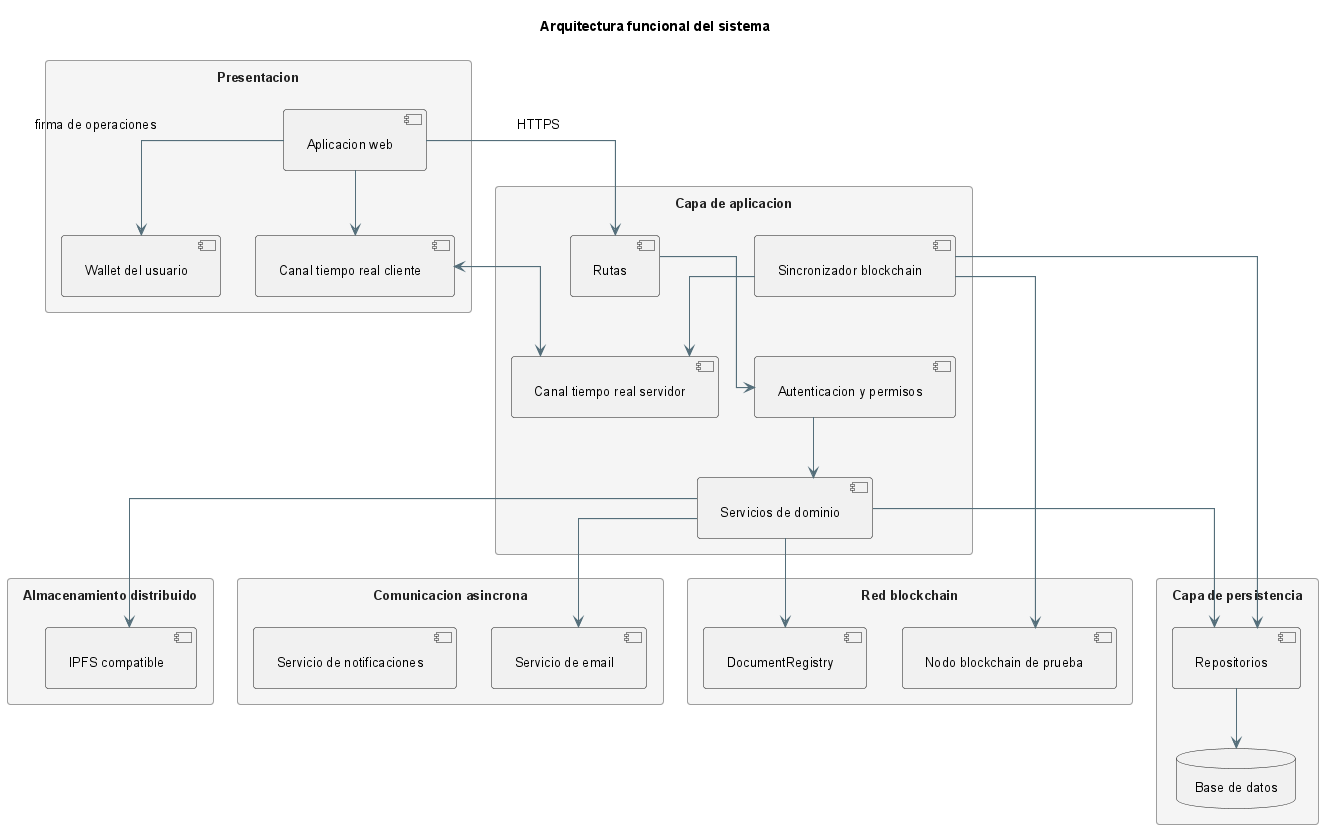
\includegraphics[width=0.95\linewidth]{diagramas/arquitectura.png}
    \caption{Arquitectura del sistema DocumentChain}
    \label{fig:arquitectura-mem}
\end{figure}

A modo de ejemplo, la Figura \ref{fig:seq-bce-ejemplo} muestra el diagrama de secuencia de analisis BCE correspondiente al caso de uso UC-0015 (Subir Documento), que ilustra la aplicacion del patron Boundary-Control-Entity. La Figura \ref{fig:seq-design-ejemplo} presenta el diagrama de secuencia de diseno para el mismo caso de uso, reflejando la implementacion real con React (frontend), Express (backend), IPFS y el smart contract.

\begin{figure}[H]
    \centering
    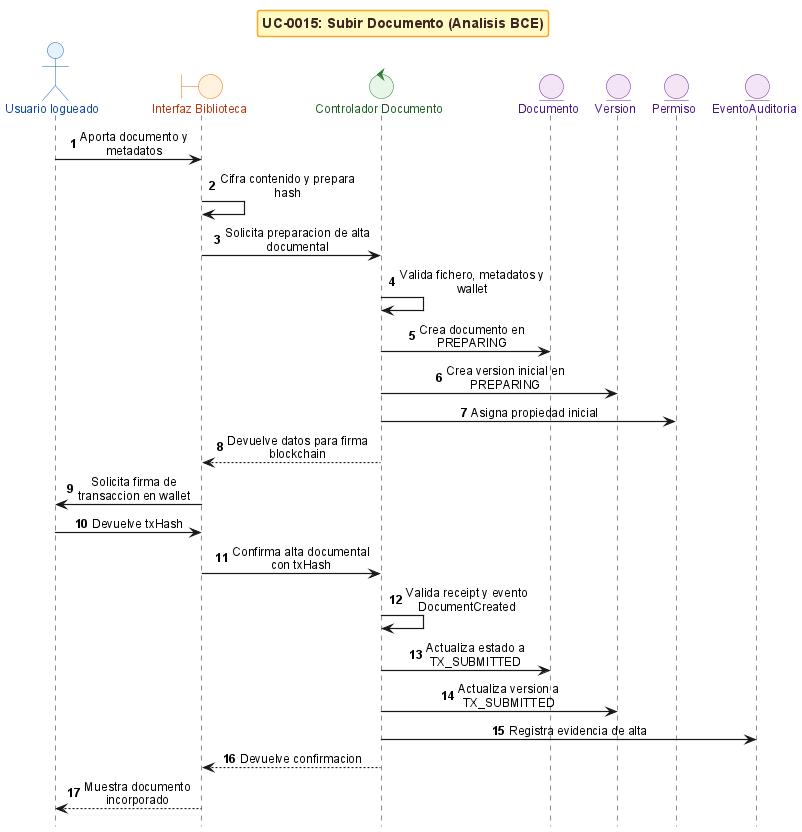
\includegraphics[width=0.92\linewidth]{diagramas/seq-bce-uc0015-upload.png}
    \caption{Diagrama de secuencia de analisis BCE: UC-0015 Subir Documento}
    \label{fig:seq-bce-ejemplo}
\end{figure}

\begin{figure}[H]
    \centering
    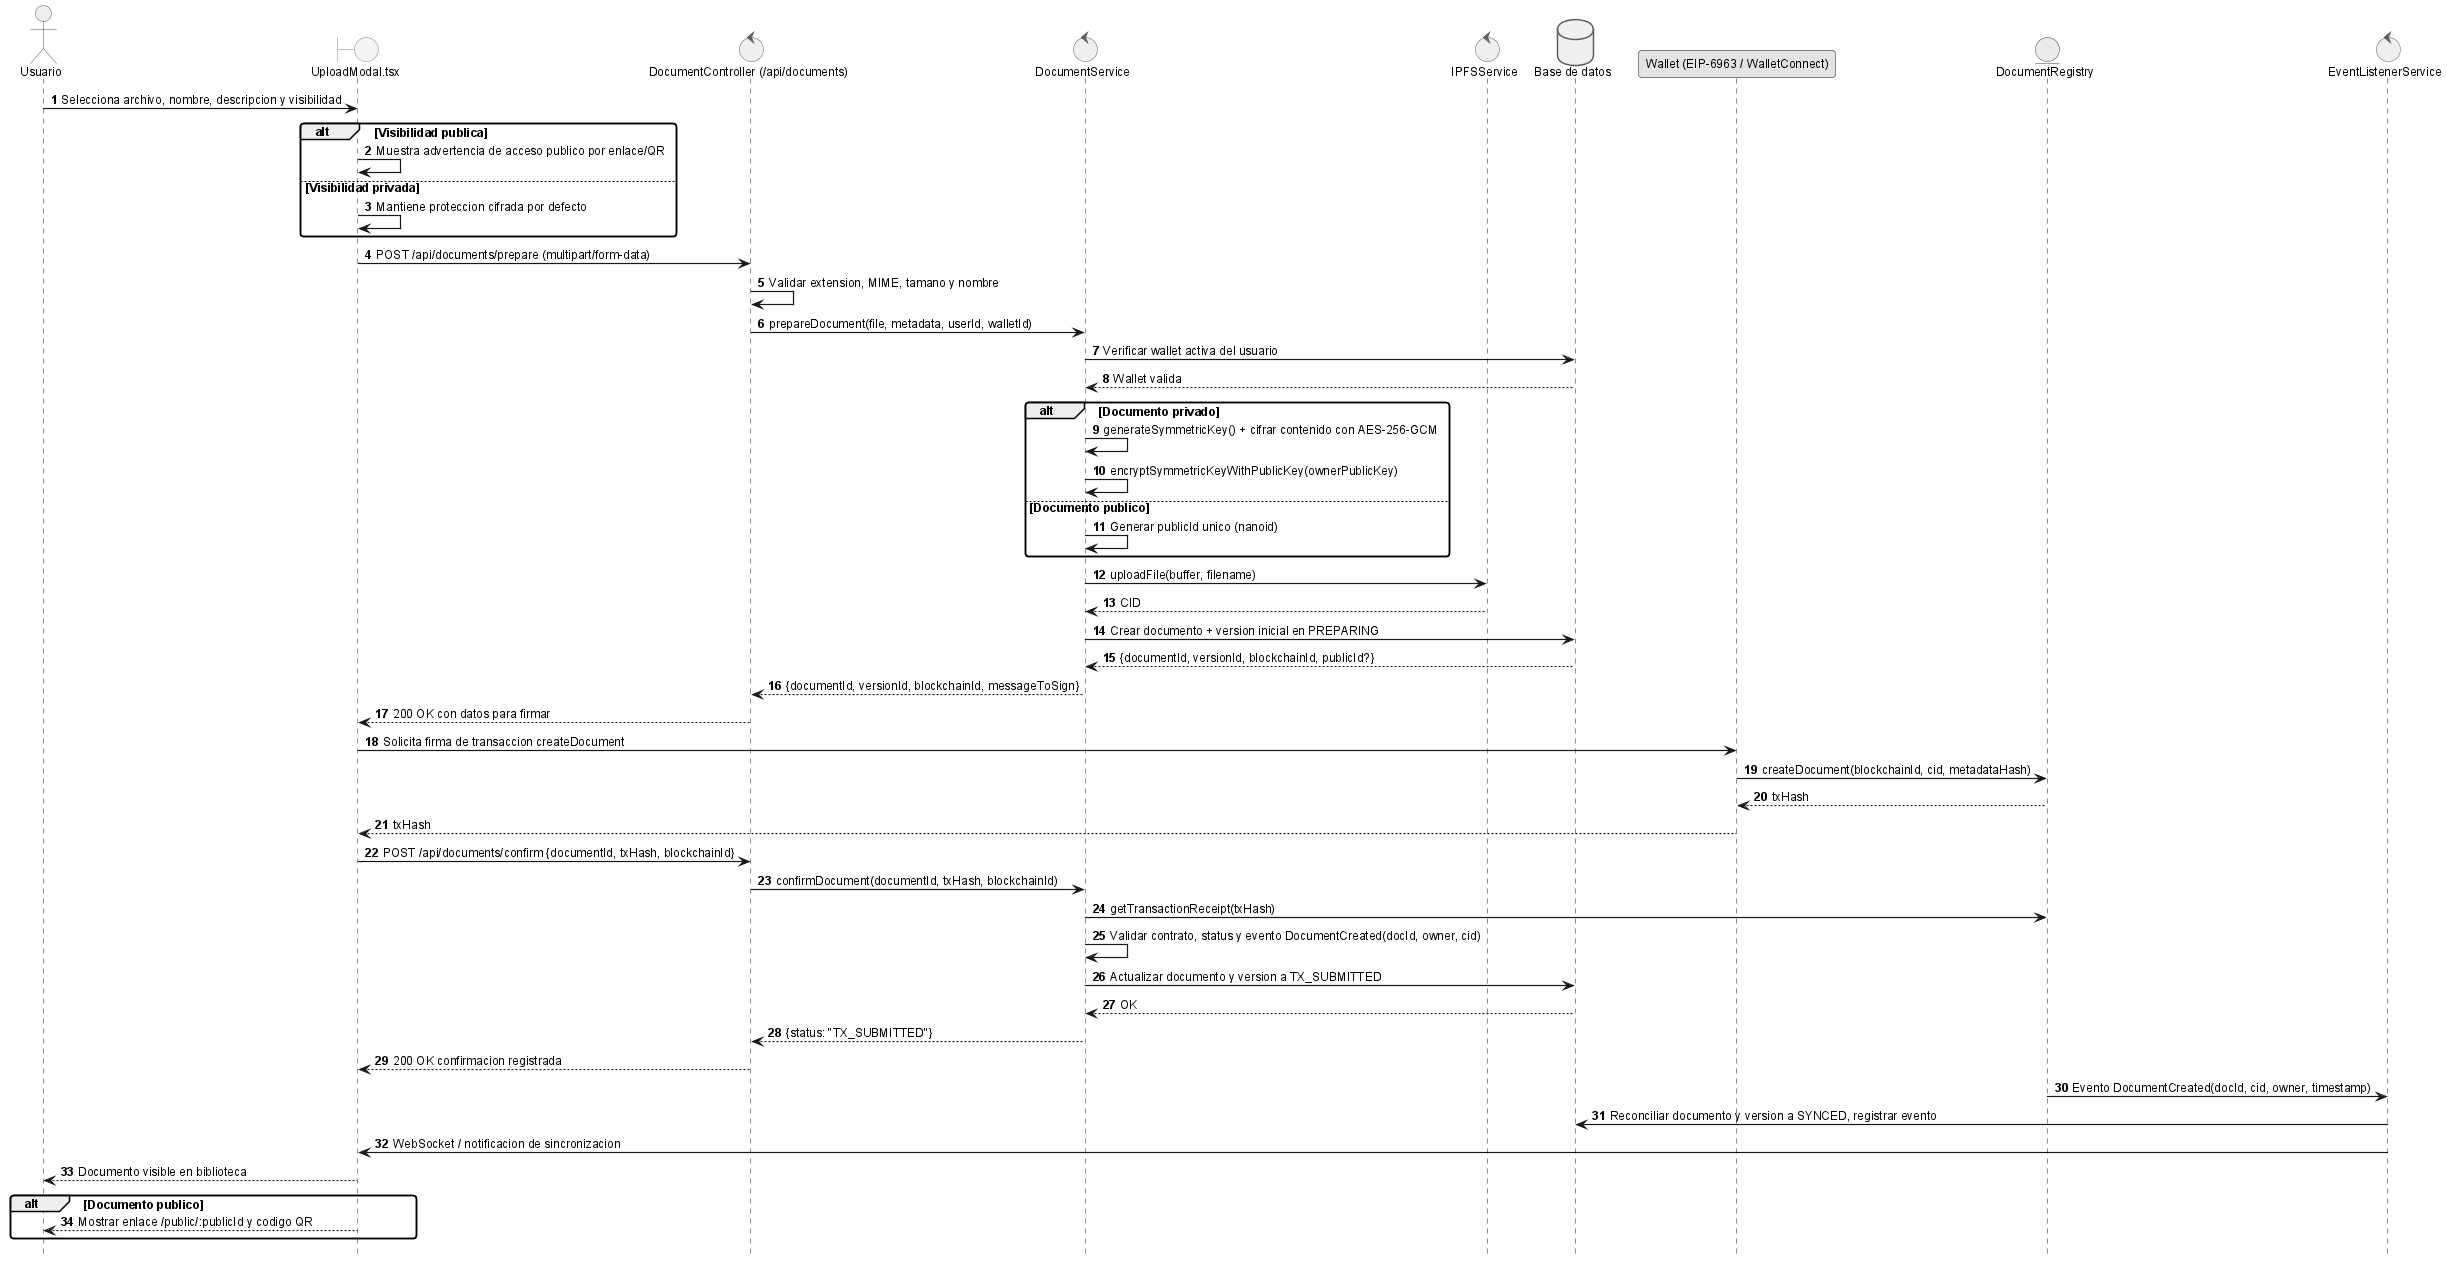
\includegraphics[width=0.92\linewidth]{diagramas/seq-upload.png}
    \caption{Diagrama de secuencia de diseno: UC-0015 Subir Documento}
    \label{fig:seq-design-ejemplo}
\end{figure}

Para obtener mas informacion sobre este apartado, consultar el Anexo III (Analisis y diseno del sistema).

\subsection{Diseno del sistema}

Una vez definidos todos los casos de uso y analizados, se procedio a disenar el sistema, preparando el proyecto para su implementacion. La arquitectura de DocumentChain se organiza en capas funcionales desacopladas, con tres subsistemas de persistencia coordinados: PostgreSQL para estado relacional mutable, IPFS para contenido binario direccionable por hash, y Ethereum para registro verificable e inmutable.

Entre las decisiones de diseno mas relevantes destacan: la eleccion de Ethereum/Hardhat frente a Hyperledger Fabric o Bitcoin por su ecosistema de herramientas y compatibilidad con wallets estandar; la adopcion de IPFS con nodo Kubo autoalojado frente al almacenamiento cloud tradicional; y la seleccion de PostgreSQL con Prisma ORM por su robustez en entornos concurrentes y su integracion con TypeScript.

El modelo de permisos on-chain distingue tres roles (VIEWER, EDITOR, OWNER) gestionados directamente por el contrato \texttt{DocumentRegistry}, y la seguridad se abordo mediante defensa en profundidad, combinando cifrado AES-256-GCM para documentos privados, proteccion de claves con criptografia asimetrica y controles de sesion en el backend.

Las Figuras \ref{fig:deployment-mem} y \ref{fig:er-mem} muestran, respectivamente, el modelo de despliegue con contenedores Docker y el diagrama entidad-relacion de la base de datos PostgreSQL. Las Figuras \ref{fig:prepare-confirm} y \ref{fig:event-listener} ilustran los dos patrones arquitectonicos fundamentales del sistema.

\begin{figure}[H]
    \centering
    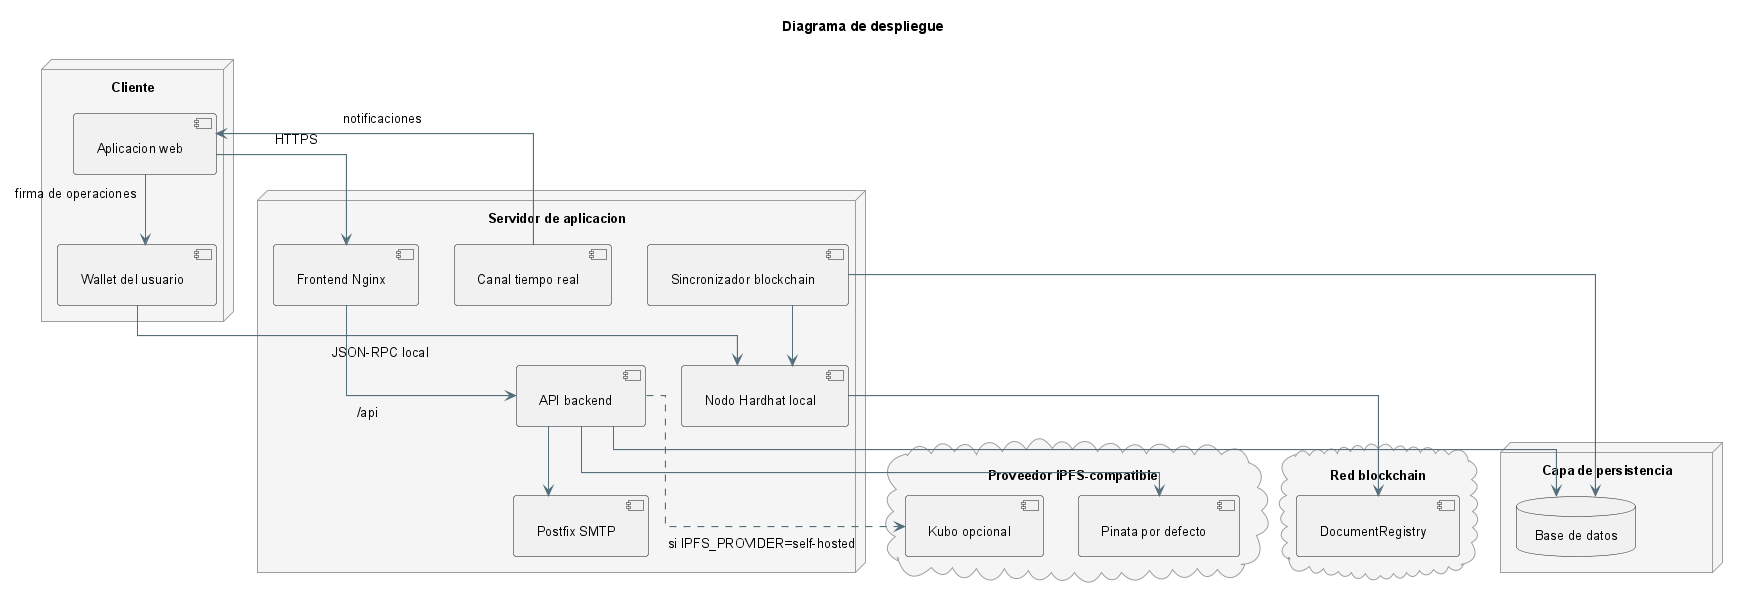
\includegraphics[width=0.95\linewidth]{diagramas/deployment.png}
    \caption{Modelo de despliegue con contenedores Docker}
    \label{fig:deployment-mem}
\end{figure}

\begin{figure}[H]
    \centering
    
\includegraphics[width=0.95\linewidth]{diagramas/er-combined.png}
    \caption{Diagrama entidad-relacion de la base de datos}
    \label{fig:er-mem}
\end{figure}

\begin{figure}[H]
    \centering
    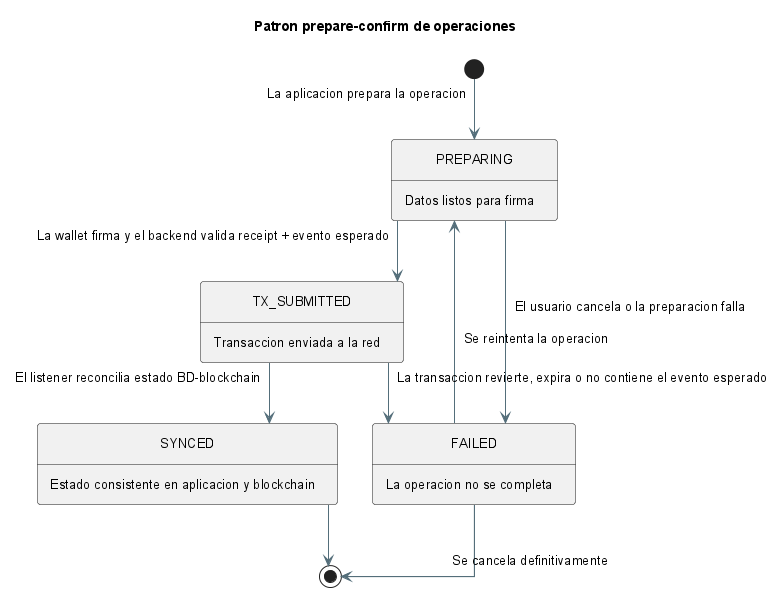
\includegraphics[width=0.88\linewidth]{diagramas/prepare-confirm.png}
    \caption{Patron prepare/confirm para transacciones blockchain}
    \label{fig:prepare-confirm}
\end{figure}

\begin{figure}[H]
    \centering
    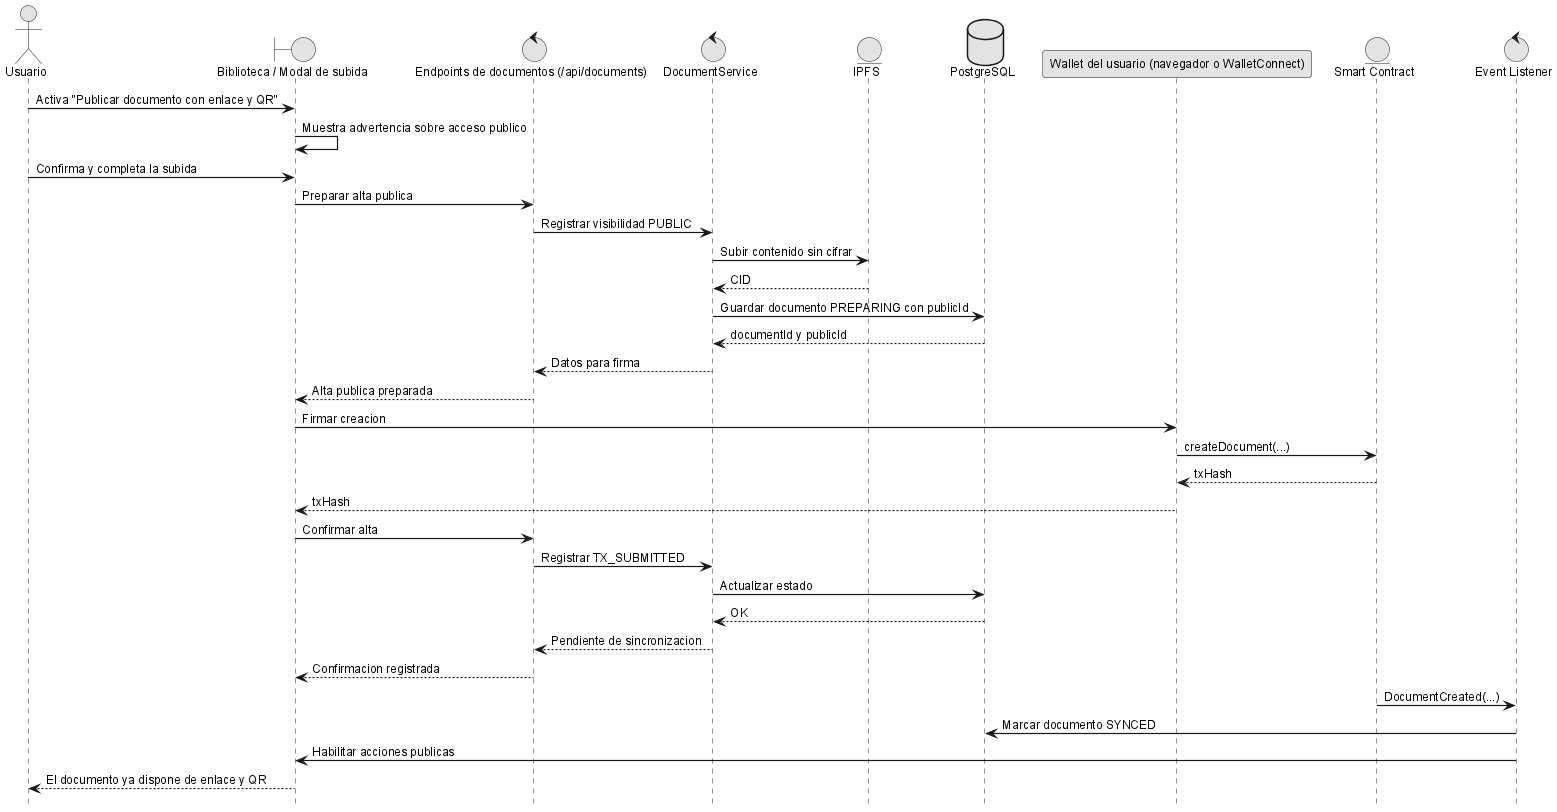
\includegraphics[width=0.90\linewidth]{diagramas/flow-public-upload.png}
    \caption{Flujo de sincronizacion bidireccional mediante Event Listener}
    \label{fig:event-listener}
\end{figure}

La Tabla \ref{tab:riesgos} resume los principales riesgos identificados y sus medidas de mitigacion.

\begin{table}[H]
\centering
\renewcommand{\arraystretch}{1.4}
\small
\begin{tabular}{|c|p{3.5cm}|c|c|p{3cm}|}
\hline
\textbf{ID} & \textbf{Riesgo} & \textbf{Prob.} & \textbf{Impacto} & \textbf{Mitigacion} \\
\hline
R-01 & Complejidad de integracion blockchain & Alta & Alto & Patron prepare/confirm; listener + worker \\
\hline
R-02 & Incompatibilidad entre wallets y EIP-6963 & Media & Medio & Soporte multicartera; fallback a WalletConnect \\
\hline
R-03 & Fallos en sincronizacion BD-blockchain & Media & Alto & Worker periodico de reconciliacion \\
\hline
R-04 & Perdida de contenido IPFS & Baja & Alto & Pin persistente de CIDs; backup periodico \\
\hline
R-05 & Vulnerabilidad en smart contract & Baja & Critico & Analisis estatico Slither; patrones OpenZeppelin \\
\hline
R-06 & Rendimiento insuficiente bajo carga & Baja & Medio & Limites de recursos; paginacion en todos los listados \\
\hline
\end{tabular}
\caption{Registro de riesgos del proyecto}
\label{tab:riesgos}
\end{table}

Para obtener mas informacion sobre este apartado, consultar el Anexo III (Analisis y diseno del sistema) y el Anexo V (Plan de seguridad).

\subsection{Implementacion}

Durante esta fase se ha realizado la codificacion de todo el sistema tomando los resultados obtenidos en la fase de diseno como base. La implementacion se dividio en cuatro secciones: servidor web (frontend React + TypeScript con Vite), servidor API (backend Node.js + Express), contratos inteligentes (Solidity + Hardhat) e infraestructura (Docker Compose).

Las decisiones tecnicas mas relevantes incluyen el diseno de una arquitectura de seguridad por capas (JWT con verificacion de email, AES-256-GCM con intercambio ECDH P-256 y registro blockchain), el flujo prepare/confirm para transacciones blockchain, la integracion de wallets mediante EIP-6963 evitando el vendor lock-in, y la sincronizacion bidireccional blockchain-base de datos mediante EventListenerService y worker de reconciliacion periodica. La contenerizacion con Docker Compose garantiza la reproducibilidad del entorno de ejecucion, orquestando siete servicios.

Para obtener mas informacion sobre este apartado, consultar el Anexo IV (Documentacion tecnica) y el Anexo VII (Manual de montaje).

\subsection{Funcionalidad del sistema}

En este apartado se muestran los aspectos mas importantes de la funcionalidad del sistema. La aplicacion dispone de un panel principal de gestion documental donde los usuarios pueden realizar todas las operaciones del ciclo de vida completo del documento, una pagina de verificacion publica accesible sin autenticacion que permite verificar la autenticidad de cualquier documento, y un panel de administracion para la gestion de usuarios, roles y supervision del sistema.

\subsubsection{Gestion documental}

La Figura \ref{fig:documents-page-mem} muestra la vista principal de gestion documental, donde los usuarios pueden listar, buscar, filtrar, subir nuevos documentos y acceder a las operaciones de cada documento (firmar, compartir, versionar, archivar, transferir). La Figura \ref{fig:upload-modal-mem} presenta el modal de subida de documentos, con campos de metadatos y seleccion de visibilidad.

\begin{figure}[H]
    \centering
    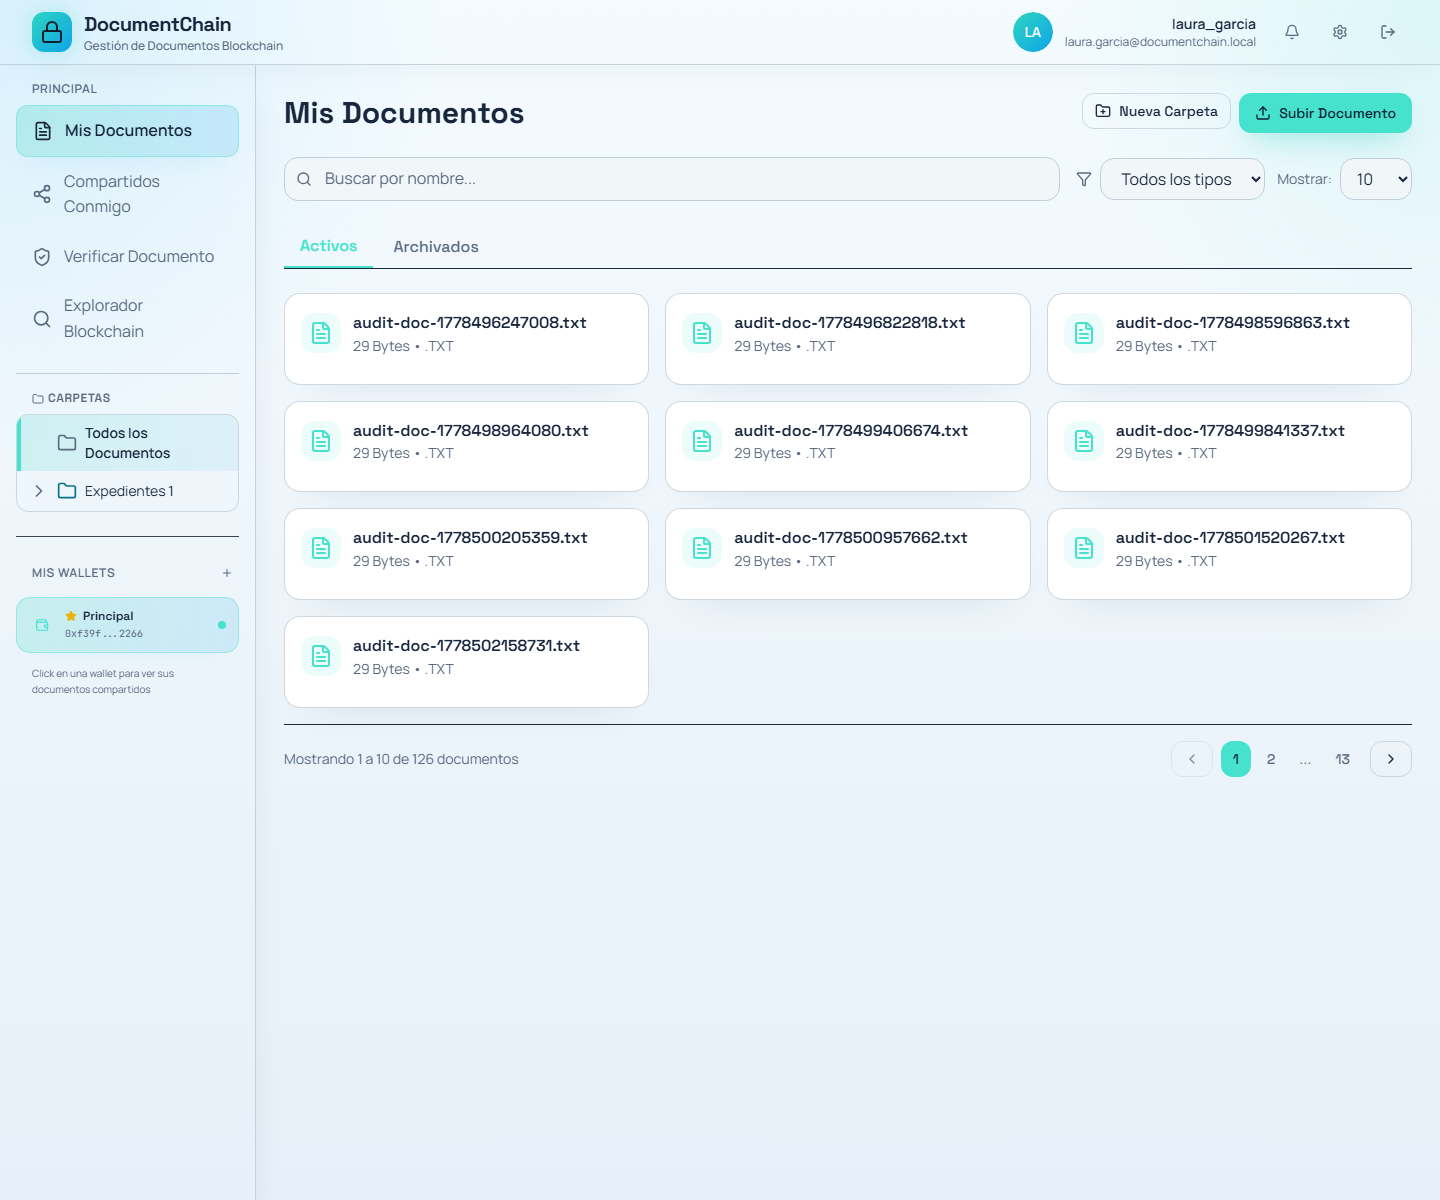
\includegraphics[width=0.95\linewidth]{capturas-ui/documents-page.png}
    \caption{Vista principal de gestion documental}
    \label{fig:documents-page-mem}
\end{figure}

\begin{figure}[H]
    \centering
    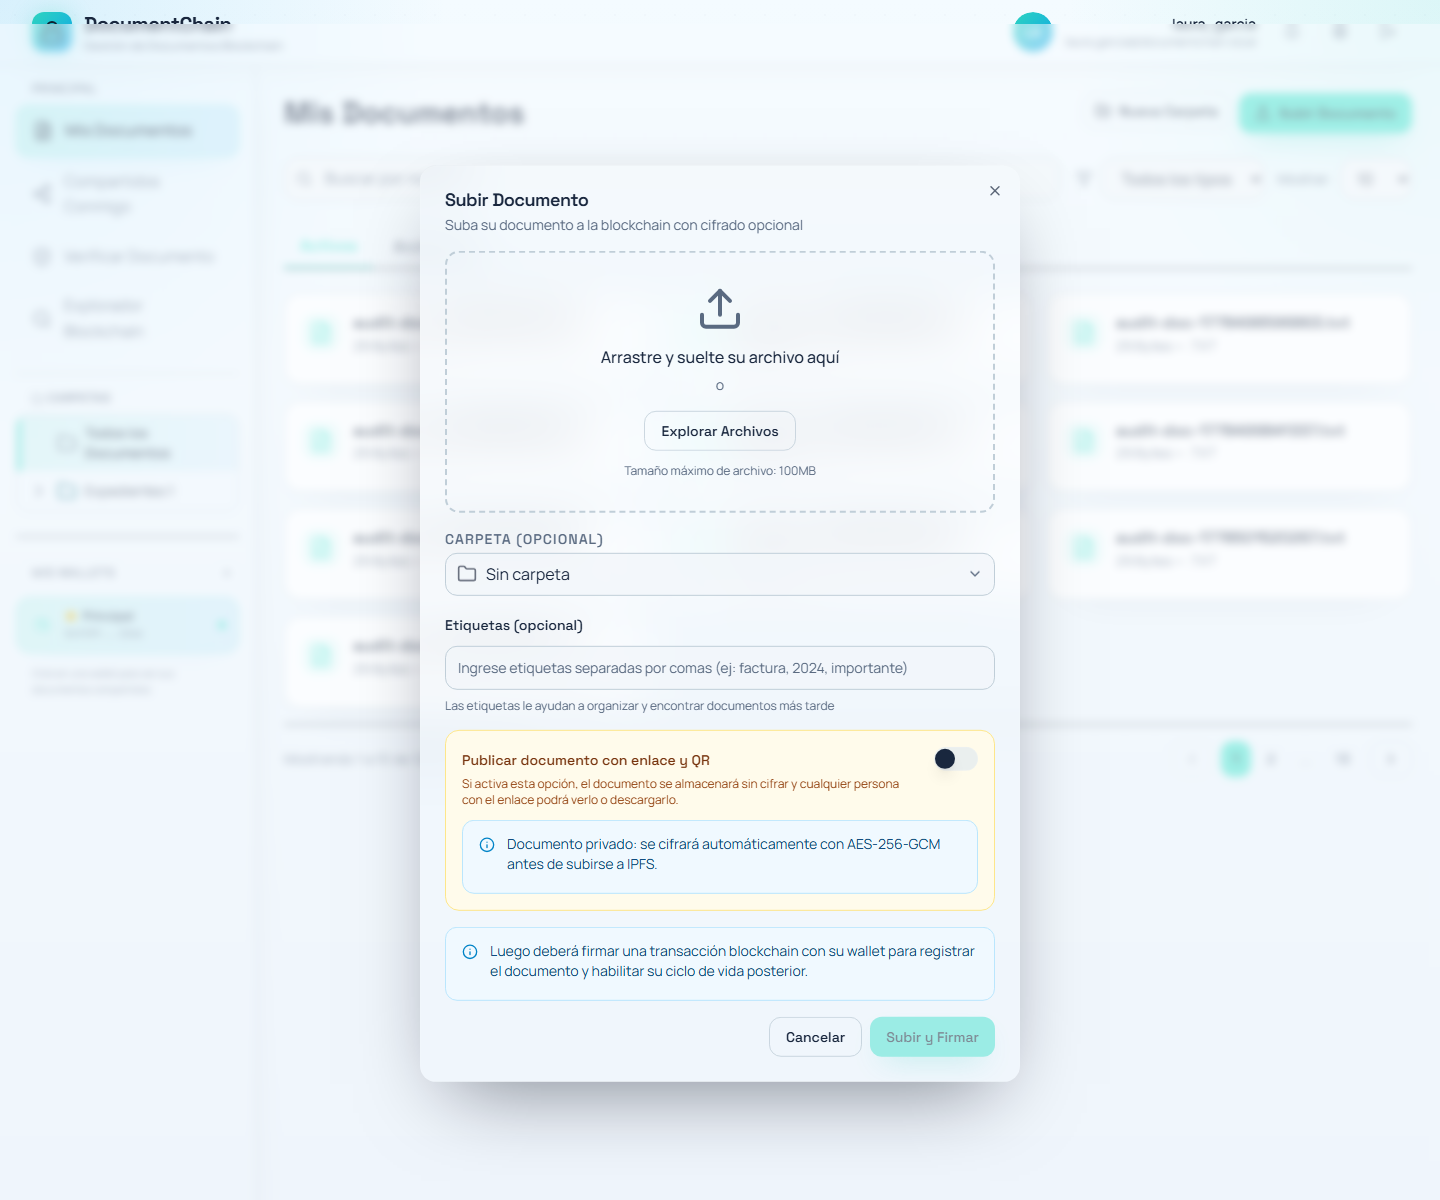
\includegraphics[width=0.85\linewidth]{capturas-ui/upload-modal.png}
    \caption{Modal de subida de documentos con metadatos}
    \label{fig:upload-modal-mem}
\end{figure}

\subsubsection{Firma digital y comparticion}

Las Figuras \ref{fig:sign-modal-mem} y \ref{fig:share-modal-mem} muestran, respectivamente, el flujo de firma digital de un documento mediante wallet blockchain y el modal de comparticion con configuracion de permisos.

\begin{figure}[H]
    \centering
    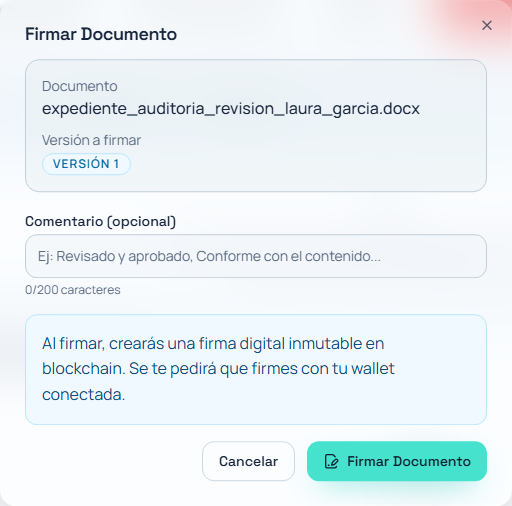
\includegraphics[width=0.85\linewidth]{capturas-ui/sign-modal.png}
    \caption{Modal de firma digital con wallet blockchain}
    \label{fig:sign-modal-mem}
\end{figure}

\begin{figure}[H]
    \centering
    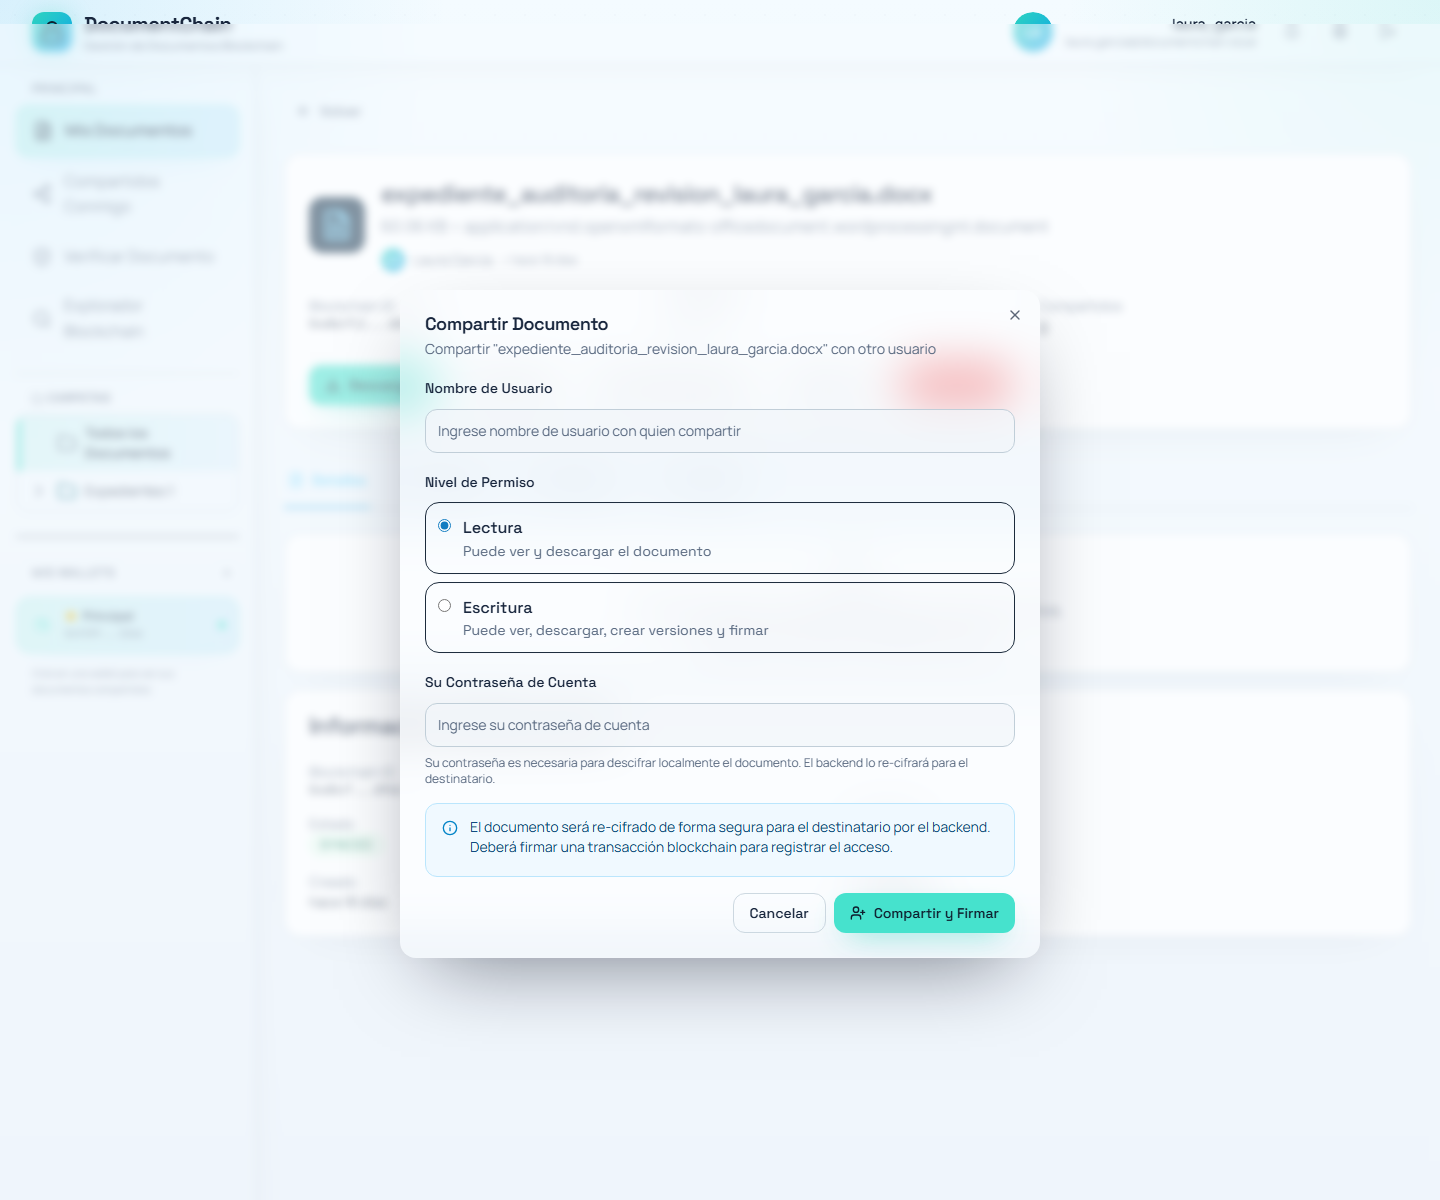
\includegraphics[width=0.85\linewidth]{capturas-ui/share-modal.png}
    \caption{Modal de comparticion de documentos con permisos}
    \label{fig:share-modal-mem}
\end{figure}

\subsubsection{Verificacion publica y administracion}

La Figura \ref{fig:verify-page-mem} muestra la pagina de verificacion publica, accesible sin necesidad de autenticacion, que permite a cualquier tercero comprobar la autenticidad de un documento mediante su hash o el identificador de la transaccion blockchain. La Figura \ref{fig:admin-dashboard-mem} presenta el panel de administracion para la gestion de usuarios y supervision del sistema.

\begin{figure}[H]
    \centering
    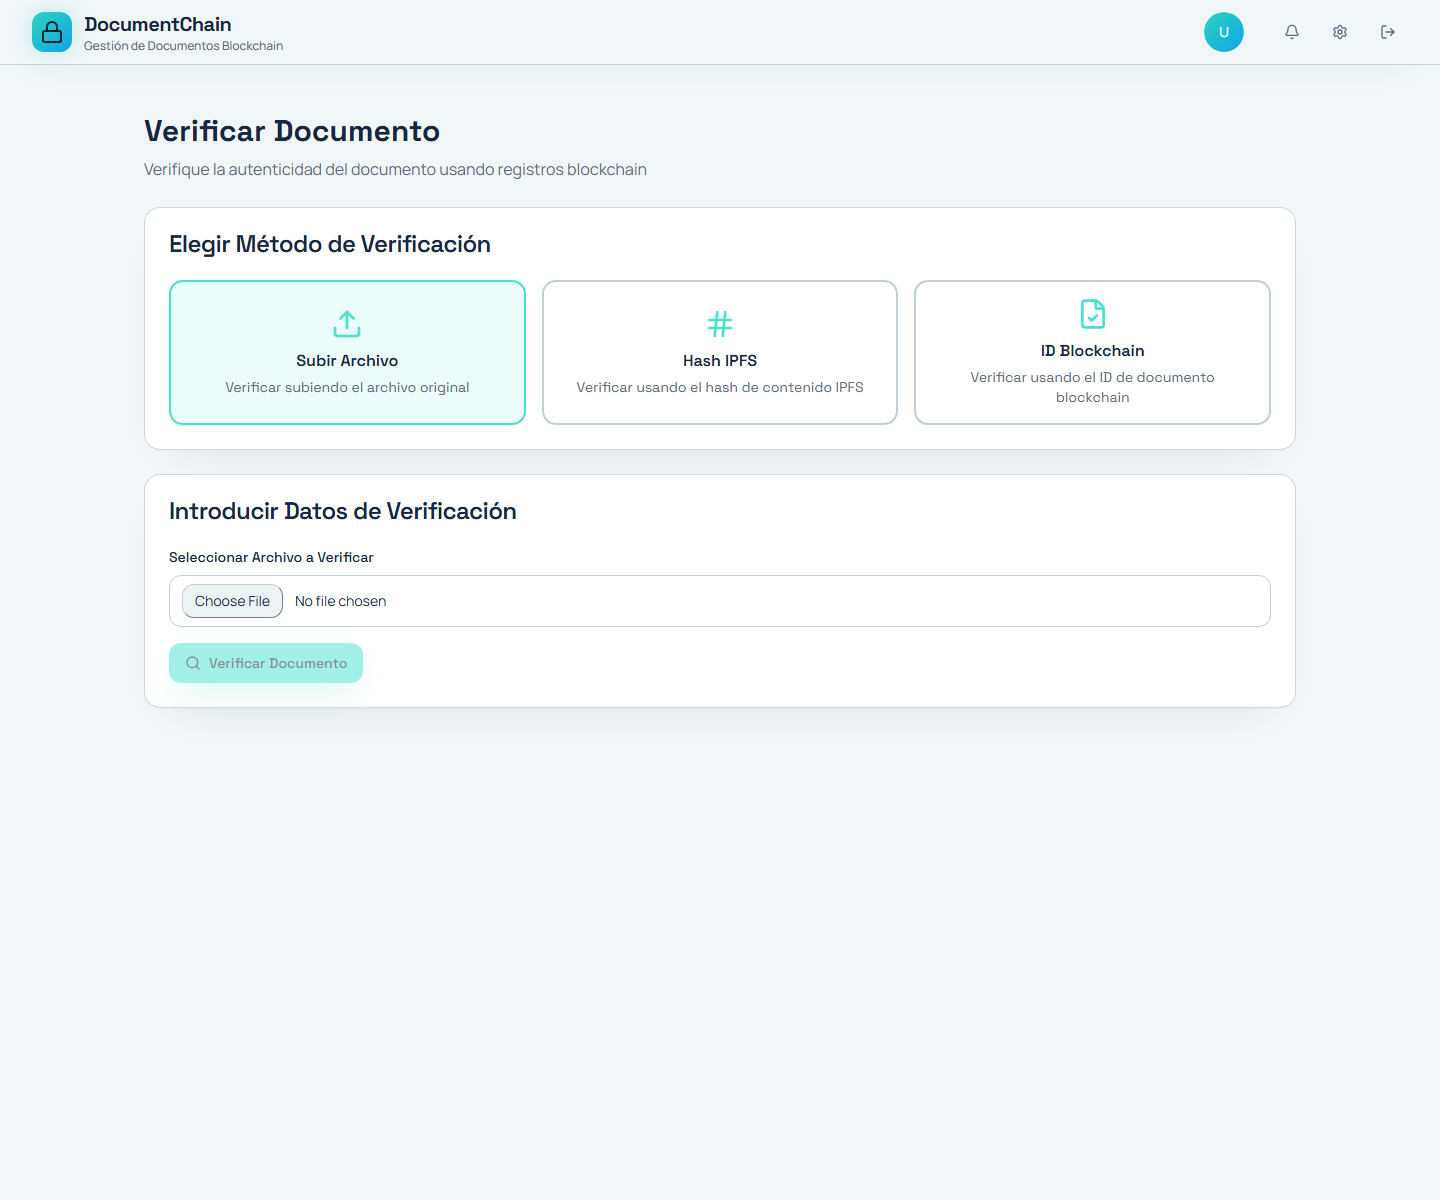
\includegraphics[width=0.92\linewidth]{capturas-ui/verify-page.png}
    \caption{Pagina de verificacion publica de autenticidad de documentos}
    \label{fig:verify-page-mem}
\end{figure}

\begin{figure}[H]
    \centering
    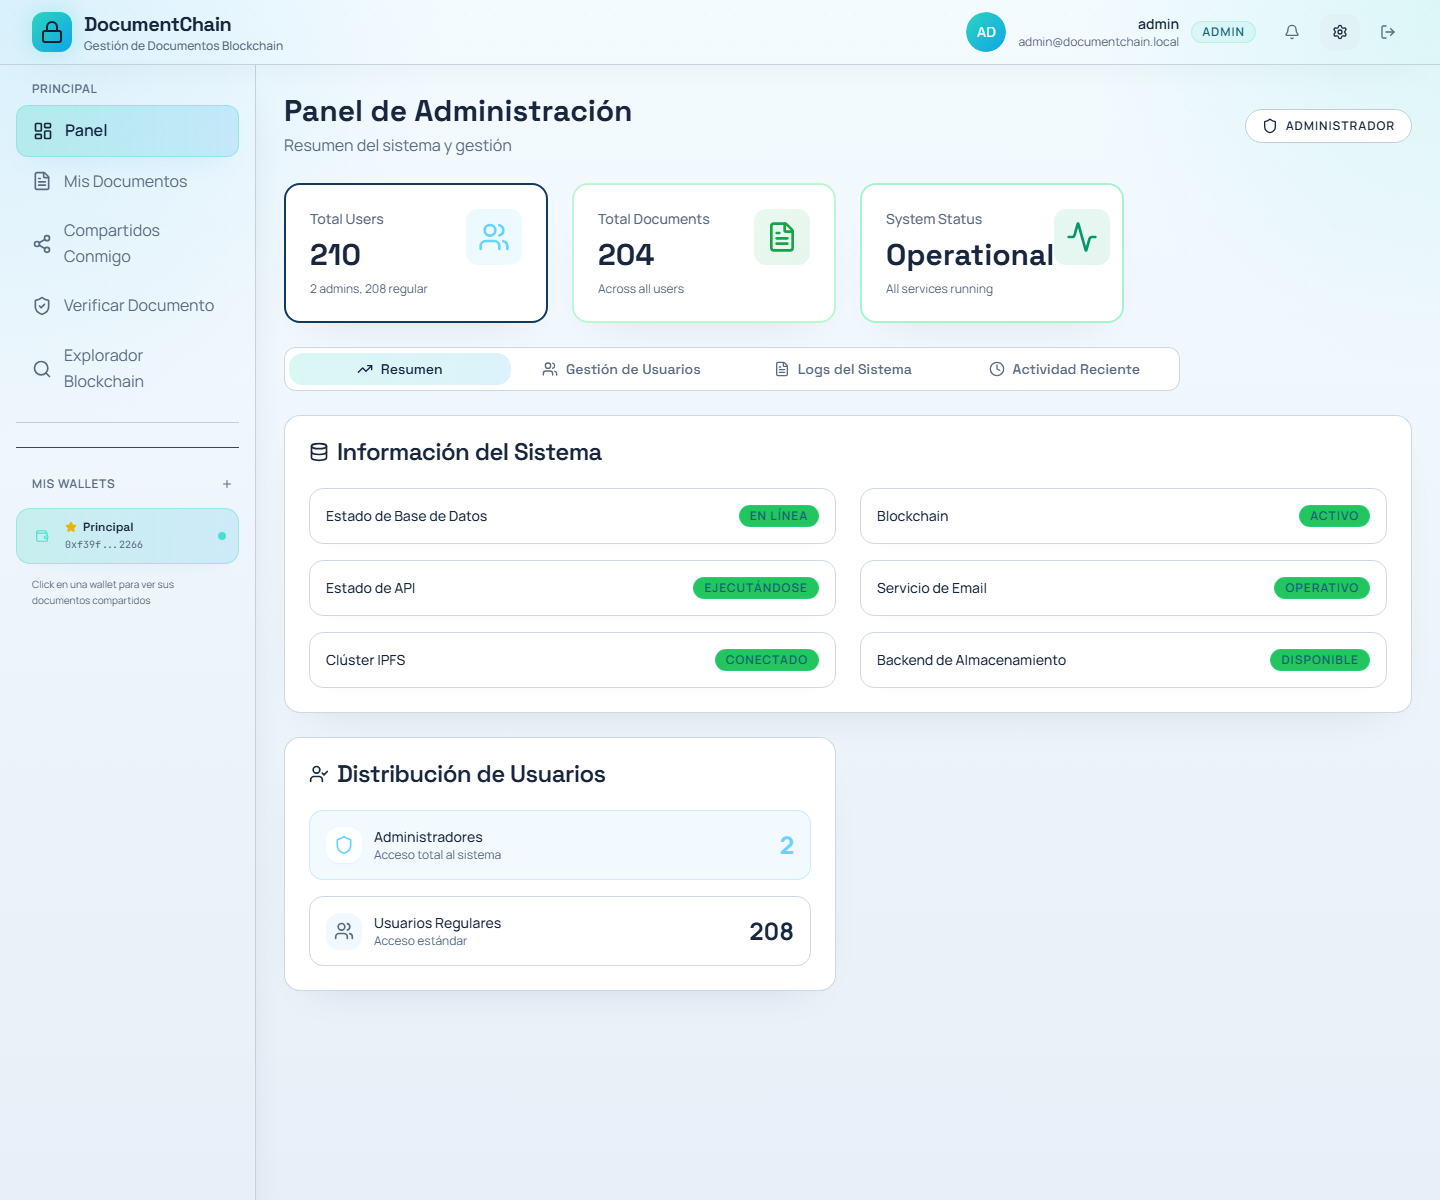
\includegraphics[width=0.95\linewidth]{capturas-ui/admin-dashboard.png}
    \caption{Panel de administracion del sistema}
    \label{fig:admin-dashboard-mem}
\end{figure}

Para obtener mas informacion sobre este apartado, consultar el Anexo VI (Manual de usuario).

% ============================================================
% CAPITULO 7: LIMITACIONES DEL SISTEMA
% ============================================================
\section{Limitaciones del sistema}

Durante el desarrollo de este proyecto se han encontrado una serie de limitaciones que condicionan su despliegue en entornos de produccion.

La Tabla \ref{tab:limitaciones-tiempo} resume las funcionalidades diferidas, su viabilidad tecnica estimada y la justificacion de su exclusion.

\begin{table}[H]
\centering
\renewcommand{\arraystretch}{1.4}
\small
\begin{tabular}{|p{4cm}|c|p{6cm}|}
\hline
\textbf{Funcionalidad diferida} & \textbf{Viabilidad} & \textbf{Justificacion de exclusion} \\
\hline
Red blockchain publica & Alta & Requiere presupuesto para gas y auditoria de seguridad \\
\hline
Notificaciones push & Alta & Dependiente de app movil; email/in-app cubren el 80\% de casos \\
\hline
App movil nativa & Media & Rediseno UI/UX completo; no port directo \\
\hline
Sistema de pagos & Alta & Proyecto empresarial independiente; no academico \\
\hline
Certificacion eIDAS & Alta & Proceso de >12 meses y coste de auditoria EEC \\
\hline
\end{tabular}
\caption{Funcionalidades diferidas por restricciones temporales}
\label{tab:limitaciones-tiempo}
\end{table}

\subsection{Restricciones tecnologicas y de infraestructura}

El sistema se ha desarrollado y probado sobre una red local de Hardhat, no sobre una blockchain real. Esto es suficiente para una demostracion, pero no refleja las condiciones de un entorno de produccion. En una red publica, cada operacion consume gas y los tiempos de confirmacion pueden variar mucho. No se ha medido como afectaria esto a la experiencia de usuario.

Otro punto debil es que el backend actual es un unico proceso. Si el sistema recibiera muchas peticiones simultaneas, probablemente se quedaria corto. Pasar a una arquitectura con varias instancias requeriria repensar como se escuchan los eventos de la blockchain para no procesar el mismo evento dos veces.

Tampoco hay un plan de copias de seguridad. PostgreSQL guarda los datos en un volumen Docker, pero si ese volumen se pierde, se pierden todos los metadatos. La blockchain conservaria los registros, pero sin los metadatos el sistema dejaria de ser util.

\subsection{Restricciones de seguridad y auditoria}

Aunque se han seguido buenas practicas de seguridad, hay que reconocer varias limitaciones importantes. El contrato inteligente no ha pasado por una auditoria profesional. Se ha usado Slither para analisis estatico y se han seguido las recomendaciones de OpenZeppelin, pero una auditoria externa encontraria casi con seguridad aspectos a mejorar.

Las pruebas de seguridad se han limitado a tests funcionales. No se han realizado pruebas de penetracion ni se han explorado vectores de ataque como front-running, manipulacion de eventos WebSocket o condiciones de carrera en el acceso a la base de datos.

Ademas, la seguridad del sistema depende de que el usuario proteja bien su contrasena y su clave de recuperacion. Si las pierde, pierde el acceso a sus documentos y el sistema no puede hacer nada al respecto, porque ni siquiera el servidor tiene acceso a las claves de cifrado.

\subsection{Acceso a usuarios y pruebas de usabilidad}

No se ha podido contar con usuarios reales para probar la aplicacion. Las pruebas se han hecho con un grupo muy reducido de personas, todas ellas con perfil tecnico, lo que introduce un sesgo importante. Conceptos como wallet, blockchain o CID, que para un informatico son familiares, pueden resultar confusos para alguien que solo quiere gestionar sus documentos.

Tampoco se han hecho pruebas A/B comparando distintos disenos, ni se ha realizado una auditoria de accesibilidad formal para comprobar que la aplicacion funciona con lectores de pantalla u otras tecnologias asistivas.

\subsection{Restricciones regulatorias y de compliance}

El RGPD establece el derecho al olvido, pero la blockchain es inmutable por diseno. Si un usuario ejerce este derecho, se puede eliminar su informacion de la base de datos, pero los hashes y las direcciones Ethereum que quedaron registrados en la cadena no se pueden borrar. Esto crea una tension que no tiene una solucion sencilla.

En cuanto al almacenamiento en IPFS, los archivos se distribuyen por nodos de todo el mundo, lo que podria entrar en conflicto con normativas que exigen que ciertos datos permanezcan dentro de un territorio concreto.

\subsection{Restricciones del proyecto}

El proyecto se ha desarrollado en unos seis meses por una unica persona, con dedicacion parcial. Esta limitacion de tiempo ha obligado a priorizar. Algunas funcionalidades que habria sido interesante incluir se quedaron fuera del alcance por este motivo, como la migracion a una red publica de pruebas, las notificaciones push nativas o un sistema de recuperacion de cuenta mas amigable para el usuario no tecnico.

% ============================================================
% CAPITULO 8: CONCLUSIONES
% ============================================================
\section{Conclusiones}

\subsection{Validacion de objetivos}

Una vez terminado el proyecto, se puede decir que los objetivos que se plantearon al principio se han cumplido. Ha sido un trabajo largo, con momentos complicados, pero el resultado es una plataforma que funciona y que demuestra que se puede hacer gestion documental con garantias blockchain sin renunciar a una experiencia de usuario razonable.

A nivel personal, el proyecto me ha permitido tocar practicamente todas las capas de una aplicacion moderna: frontend con React, backend con Node.js, base de datos con PostgreSQL, almacenamiento descentralizado con IPFS y, por supuesto, blockchain con Solidity. Muchas de estas tecnologias las conoci durante la carrera, pero nunca las habia integrado en un mismo sistema. Ha sido un aprendizaje intenso.

Tambien he podido aplicar metodologias de ingenieria del software que habia estudiado en asignaturas como Ingenieria del Software (Proceso Unificado, UML) o Gestion de Proyectos (Use Case Points, planificacion con Gantt). Ver como los diagramas de casos de uso se transforman en endpoints REST y como una estimacion en horas se convierte en un calendario real ha sido de las partes mas satisfactorias del proyecto.

La Tabla \ref{tab:validacion-obj} resume que tal ha ido cada objetivo.

\begin{table}[H]
\centering
\renewcommand{\arraystretch}{1.4}
\small
\begin{tabular}{|c|p{8cm}|c|}
\hline
\textbf{Objetivo} & \textbf{Descripcion} & \textbf{Estado} \\
\hline
OBJ-0001 & Gestionar ciclo de vida completo de documentos (crear, versionar, compartir, firmar, archivar, eliminar) & Alcanzado \\
\hline
OBJ-0002 & Garantizar autenticidad e integridad mediante registro inmutable en blockchain & Alcanzado \\
\hline
OBJ-0003 & Firma digital con wallets blockchain compatibles EIP-6963 & Alcanzado \\
\hline
OBJ-0004 & Comparticion controlada con permisos on-chain (VIEWER, EDITOR, OWNER) & Alcanzado \\
\hline
OBJ-0005 & Auditoria publica de transacciones mediante endpoint por txHash & Alcanzado \\
\hline
OBJ-0006 & Confidencialidad con cifrado de extremo a extremo (AES-256-GCM + ECDH) & Alcanzado \\
\hline
OBJ-0007 & Gestion de multiples wallets con identificacion mediante EIP-6963 & Alcanzado \\
\hline
OBJ-0008 & Panel de administracion con gestion de usuarios, roles y supervision del sistema & Alcanzado \\
\hline
\end{tabular}
\caption{Validacion de objetivos funcionales}
\label{tab:validacion-obj}
\end{table}

Mas alla de los objetivos concretos, creo que el trabajo aporta algo interesante: una arquitectura documentada que separa lo que necesita ser inmutable (blockchain) de lo que necesita ser rapido (PostgreSQL, IPFS). No es una idea nueva, pero tenerla implementada y explicada paso a paso, con diagramas, manuales y codigo fuente, puede servir como referencia para otros estudiantes o desarrolladores que quieran explorar este camino.

Para mas detalle sobre la planificacion y como se ajusto a lo estimado, se puede consultar el Anexo II.

% ============================================================
% CAPITULO 9: LINEAS DE TRABAJO FUTURAS
% ============================================================
\section{Lineas de trabajo futuras}

Ya que ningun diseno es perfecto, se plantean una serie de ideas para mejorar el sistema:

\begin{itemize}
    \item \textbf{Migracion a redes blockchain publicas}: desplegar el contrato DocumentRegistry en una red de pruebas publica (Sepolia) y, tras auditoria de seguridad profesional, migrar a una red principal o Layer 2 (Polygon, Arbitrum) con un sistema de meta-transacciones para eliminar la barrera del gas para el usuario final.
    \item \textbf{Aplicacion movil nativa o PWA}: desarrollar una aplicacion para iOS/Android o convertir el frontend actual en una Progressive Web App instalable, con almacenamiento seguro de claves y notificaciones push nativas.
    \item \textbf{Mejoras de usabilidad}: implementar un tour interactivo guiado para nuevos usuarios, modelo de cuenta abstracta (ERC-4337) para abstraer la complejidad de las wallets, y visores de documentos integrados en la interfaz.
    \item \textbf{Funcionalidades avanzadas}: firma colectiva multisig con umbrales de firmantes, plantillas de documentos personalizables, flujos de aprobacion configurables y busqueda semantica sobre el contenido textual de los documentos.
    \item \textbf{Sostenibilidad del proyecto}: publicar el codigo bajo licencia open source (MIT), mantener documentacion OpenAPI actualizada y establecer un programa de recompensas por bugs.
\end{itemize}

% ============================================================
% CAPITULO 10: REFERENCIAS Y BIBLIOGRAFIA
% ============================================================
\section{Referencias y bibliografia}

\begin{enumerate}
    \item Karner, G. (1993). ``Resource Estimation for Objectory Projects''. Objective Systems SF AB.
    \item Nakamoto, S. (2008). ``Bitcoin: A Peer-to-Peer Electronic Cash System''.
    \item Wood, G. (2014). ``Ethereum: A Secure Decentralised Generalised Transaction Ledger''. Ethereum Project Yellow Paper.
    \item Benet, J. (2014). ``IPFS - Content Addressed, Versioned, P2P File System''. arXiv:1407.3561.
    \item Loshin, P. (2013). ``IPv6 Addressing and Subnetting''. John Wiley \& Sons.
    \item INCIBE (2023). ``Plan Director de Seguridad''. Instituto Nacional de Ciberseguridad.
    \item OWASP Foundation (2021). ``OWASP Top 10:2021''.
    \item React Documentation (2025). ``React 19 Documentation''. Meta Platforms.
    \item Prisma Documentation (2025). ``Prisma ORM Documentation''. Prisma Data.
    \item Hardhat Documentation (2025). ``Hardhat Documentation''. Nomic Foundation.
    \item IEEE (2019). ``IEEE Reference Guide''. IEEE Author Center.
    \item Union Europea (2014). ``Reglamento (UE) n.° 910/2014 del Parlamento Europeo y del Consejo, de 23 de julio de 2014, relativo a la identificacion electronica y los servicios de confianza para las transacciones electronicas en el mercado interior (eIDAS)''. Diario Oficial de la Union Europea, L 257/73.
    \item Union Europea (2016). ``Reglamento (UE) 2016/679 del Parlamento Europeo y del Consejo, de 27 de abril de 2016, relativo a la proteccion de las personas fisicas en lo que respecta al tratamiento de datos personales y a la libre circulacion de estos datos (RGPD)''. Diario Oficial de la Union Europea, L 119/1.
    \item ACFE (2024). ``Occupational Fraud 2024: A Report to the Nations''. Association of Certified Fraud Examiners.
    \item Buterin, V. (2014). ``Ethereum: Platform Review''. Opportunities and Challenges for Private and Consortium Blockchains.
    \item Antonopoulos, A. M., \& Wood, G. (2018). ``Mastering Ethereum: Building Smart Contracts and DApps''. O'Reilly Media.
    \item Wohrer, M., \& Zdun, U. (2018). ``Smart Contracts: Security Patterns in the Ethereum Ecosystem and Solidity''. International Workshop on Blockchain Oriented Software Engineering (IWBOSE).
    \item Merkle, R. C. (1980). ``Protocols for Public Key Cryptosystems''. IEEE Symposium on Security and Privacy.
    \item Daemen, J., \& Rijmen, V. (2002). ``The Design of Rijndael: AES - The Advanced Encryption Standard''. Springer.
    \item Swartz, A. (2014). ``Bitcoin: Its History, Technology and Governance''. Communications of the ACM, 57(7).
    \item OpenZeppelin (2023). ``OpenZeppelin Contracts Documentation v5.0''. OpenZeppelin Community.
    \item Trail of Bits (2023). ``Smart Contract Security Field Guide''. Trail of Bits, Inc.
    \item Docker Inc. (2024). ``Docker Documentation: Compose File Specification''. Docker, Inc.
    \item Mozilla Developer Network (2024). ``Web Crypto API Documentation''. MDN Web Docs.
    \item Zyskind, G., Nathan, O., \& Pentland, A. (2015). ``Decentralizing Privacy: Using Blockchain to Protect Personal Data''. IEEE Security and Privacy Workshops.
    \item Liang, X., Shetty, S., Tosh, D., Kamhoua, C., Kwiat, K., \& Njilla, L. (2017). ``ProvChain: A Blockchain-based Data Provenance Architecture in Cloud Environment with Enhanced Privacy and Availability''. IEEE/ACM CCGrid.
    \item Ateniese, G., Magri, B., Venturi, D., \& Andrade, E. (2017). ``Redactable Blockchain -- or -- Rewriting History in Bitcoin and Friends''. IEEE European Symposium on Security and Privacy.
    \item Brooke, J. (1996). ``SUS: A Quick and Dirty Usability Scale''. Usability Evaluation in Industry. Taylor \& Francis.
    \item Bangor, A., Kortum, P., \& Miller, J. (2009). ``Determining What Individual SUS Scores Mean: Adding an Adjective Rating Scale''. Journal of Usability Studies, 4(3).
    \end{enumerate}

\end{document}
